%%%%%%%%%%%%%%%%%%%%%%%%%%%%%%%%%%%%%%%%%%%%%%%%%%%%%%%%%%%%%%%%%%%
%                                                                 %
%                 Packages / Grundeinstellungen                   %
%                                                                 %
%%%%%%%%%%%%%%%%%%%%%%%%%%%%%%%%%%%%%%%%%%%%%%%%%%%%%%%%%%%%%%%%%%%

% Erstellen eines PDF/A 4 
\DocumentMetadata{
    pdfversion=2.0,
    pdfstandard=A-4,
}

% Festlegung des Allgemeinen Dokumentenformat
\documentclass[a4paper,12pt,parskip=half,headsepline,DIV=12,numbers=noenddot]{scrartcl}

%%%%%% Muss in die documentclass %%%%%%%%
%BCOR=12mm, Korrektur fuer die Bindung
%DIV12 DIV-Wert fuer die Erstellung des Satzspiegels

% Keine floats in andere Sections
\usepackage[section]{placeins}

% Weitere Pakete
\usepackage{microtype}
\usepackage{caption}
\usepackage{fontspec}
\usepackage{pdflscape}
\usepackage{float}
\usepackage{dirtree}
\usepackage{subcaption}
\usepackage{enumitem}

% Booktabs Tabellen
\usepackage{tabularray}
\UseTblrLibrary{booktabs}
\DefTblrTemplate{contfoot-text}{normal}{Fortsetzung auf nächster Seite}
\SetTblrTemplate{contfoot-text}{normal}
\DefTblrTemplate{conthead-text}{normal}{}
\SetTblrTemplate{conthead-text}{normal}

% Um Captions in Tabellen zu deaktivieren 
%\DefTblrTemplate{caption-tag}{default}{}
%\DefTblrTemplate{caption-sep}{default}{}
%\DefTblrTemplate{caption-text}{default}{}

% Grafiken aus PNG Dateien einbinden
\usepackage{graphicx}

% Deutsche Sonderzeichen und Silbentrennung nutzen
\usepackage[ngerman]{babel}
\usepackage{blindtext}

% Eurozeichen einbinden
\usepackage[right]{eurosym}

% Kopf- und Fußzeilen
\usepackage[headsepline,autooneside=false]{scrlayer-scrpage}
\clearpairofpagestyles

% Schriftart 
\usepackage{lmodern}
\setmainfont{TeX Gyre Termes}
\setsansfont{TeX Gyre Adventor}

% Floatende Bilder ermöglichen
\usepackage{floatflt}

% tikz
\usepackage{tikz}
\usetikzlibrary{calc,arrows,math}
\usetikzlibrary{shapes.geometric,positioning}

%% Schaltpläne nach europäischen Richtlinien
\usepackage[european]{circuitikz}
\tikzset{x=1mm,y=1mm}

\usepackage{siunitx}
\sisetup{output-decimal-marker={,},detect-all}

% Bricht lange URLs "schön" um
\usepackage[hyphens,obeyspaces,spaces]{url}

% Paket für Textfarben
\usepackage{xcolor} 
\definecolor{LightGray}{gray}{0.9}
\usepackage[pagecolor=white]{pagecolor}

% Mathematische Symbole importieren
\usepackage{amssymb}

% Paket für Zeilenabstand
\usepackage{setspace}

% Für Bildbezeichner
\usepackage{capt-of}

% Für Stichwortverzeichnis
\usepackage{makeidx}

% Für if und while 
\usepackage{etoolbox}

% Konfiguriere das Inhaltsverzeichnis
\usepackage{tocbasic}
\DeclareTOCStyleEntries[
  raggedentrytext,
  %numwidth=0pt, if numbers=noenddot is not set
  numsep=1ex,
  dynnumwidth,
]{tocline}{chapter,section}
\DeclareTOCStyleEntries[
  linefill=\TOCLineLeaderFill,
]{tocline}{section,subsection,subsubsection,paragraph,subparagraph}

\newcommand*\tocentryformat[1]{{\rmfamily#1}}
\RedeclareSectionCommands
  [tocentryformat=\tocentryformat,tocpagenumberformat=\tocentryformat]{subsection,subsubsection,paragraph,subparagraph}

\newcommand*\tocentrysectionformat[1]{{\rmfamily\bfseries#1}}
\RedeclareSectionCommands
  [tocentryformat=\tocentrysectionformat,tocpagenumberformat=\tocentrysectionformat]{section}  
  
\DeclareTOCStyleEntries[
  pagenumberbox=\hbox,
  dynnumwidth]{tocline}{chapter,section,subsection,subsubsection,paragraph,subparagraph,figure,table}

% Für schönere Listings
\usepackage[newfloat,]{minted}
\setminted{
  frame=lines,
  framesep=2mm,
  baselinestretch=1.2,
  bgcolor=LightGray,
  fontsize=\footnotesize,
  linenos,
  breaklines=true,
  breakanywhere=true,
  autogobble,
  tabsize=2
}
\setmintedinline{}

% Keine Floats bei Listings
\newenvironment{code}[2]
  {\captionsetup{type=listing}
  \providecommand{\captiontitle}{#1}
  \providecommand{\labeltitle}{#2}
  \vspace*{0.3cm}
  }
  {
  \vspace*{-0.8cm}
  \caption{\captiontitle}
  \label{\labeltitle}
  \vspace*{0.35cm}
  }
\SetupFloatingEnvironment{listing}{}

% Nummerierung inkl. Section
\usepackage{chngcntr}
\counterwithin{table}{section}
\counterwithin{figure}{section}
\counterwithin{listing}{section}

% Abkürzungsverzeichnis
\usepackage[printonlyused, smaller, withpage]{acronym}

% Erzeugt Inhaltsverzeichnis mit Querverweisen zu den Abschnitten (PDF Version)
\usepackage[bookmarksnumbered,hyperfootnotes=false,hypertexnames=false]{hyperref}
\hypersetup{
    colorlinks=true,
    linkcolor=black,
    filecolor=blue,
    citecolor = black,      
    urlcolor=blue,
}

% Darf erst hier eingebunden werden! 
\usepackage{subfiles}
\usepackage{csquotes}

% Indexerstellung
\makeindex


%%%%%%%%%%%%%%%%%%%%%%%%%%%%%%%%%%%%%%%%%%%%%%%%%%%%%%%%%%%%%%%%%%%
%                                                                 %                    
%                   Definition Zitierstil                         %
%                                                                 %
%%%%%%%%%%%%%%%%%%%%%%%%%%%%%%%%%%%%%%%%%%%%%%%%%%%%%%%%%%%%%%%%%%%

% Zitierung nach IEEE

\usepackage[
backend=biber,
style=ieee,
autocite=inline,
]{biblatex}
\addbibresource{bibtex/hauptdatei.bib}

% Zitierung nach APA

%\usepackage[
%backend=biber,
%style=apa,
%autocite=inline,
%]{biblatex}
%\addbibresource{bibtex/hauptdatei.bib}

\setcounter{biburllcpenalty}{7000}
\setcounter{biburlucpenalty}{8000}
%%%%%%%%%%%%%%%%%%%%%%%%%%%%%%%%%%%%%%%%%%%%%%%%%%%%%%%%%%%%%%%%%%%
%                                                                 %                    
%                    Definition Deckblatt                         %
%                                                                 %
%%%%%%%%%%%%%%%%%%%%%%%%%%%%%%%%%%%%%%%%%%%%%%%%%%%%%%%%%%%%%%%%%%%

% true für Bachelorarbeit / false für Hausarbeit
\newbool{bachelorarbeit}
\setbool{bachelorarbeit}{false}

% Setze Fachbereich
\newcommand{\department}{Fachbereich II \\ Management und Informationssysteme}

% Setze Studiengang
\newcommand{\studyprogram}{Wirtschaftsinformatik B.Sc.}

% Setze Modulname (bachelorarbeit muss false sein)
\newcommand{\modulname}{Qualitätsmanagement}

% Setze Dozent:in (bachelorarbeit muss false sein)
\newcommand{\auditor}{\textbf{Dozent:in:} \> Prof. Dr. Karin Vosseberg}

% Setze Gutachter:innen (bachelorarbeit muss true sein)
\newcommand{\firstauditor}{\textbf{Erstgutachter:} \> Prof. Dr. Maxi Mustermann}
\newcommand{\secondauditor}{\textbf{Zweitgutachterin:} \> Prof. Dr. Maxi Musterfrau}

% Setze Titel und Untertitel der Abreit 
\newcommand{\thetitle}{Semesteraufgabe}
\newcommand{\thesubtitle}{Entwicklung einer Hausverwaltung}

% Setze Autor:in und MatNr.
\newcommand{\theauthor}{Junior Lesage Ekane Njoh}
\newcommand{\matriculationnumber}{40128}

% Abstand zwischen Name und MatNr. (siehe Deckblatt)
\newcommand{\myspace}{1.0cm}

% Muss in src/basic_structure/deckblatt.tex einkommentiert werden! 

\newcommand{\secondauthor}{\> Steve Aguiwo II \> MatNr. 40088\\}
\newcommand{\thirdauthor}{\> Franck Majeste Dogmo Silatsa \> MatNr. 00000\\}
\newcommand{\fourthauthor}{\> Maxi Mustermensch \> MatNr. 00000\\}
\newcommand{\fifthauthor}{\> Maxi Mustermensch \> MatNr. 00000\\}

% PDF Metadaten
%\hypersetup{pdfinfo={
%Title={\thetitle},
%Author={\theauthor}
%}}

\hypersetup{pdfinfo={
Title={\thetitle},
Author={\theauthor}
}}

%%%%%%%%%%%%%%%%%%%%%%%%%%%%%%%%%%%%%%%%%%%%%%%%%%%%%%%%%%%%%%%%%%%
%                                                                 %                    
%                     Beginn des Inhalts                          %
%                                                                 %
%%%%%%%%%%%%%%%%%%%%%%%%%%%%%%%%%%%%%%%%%%%%%%%%%%%%%%%%%%%%%%%%%%%

%%%%%%%%%%%%%%%%%%%%%%%%%%%%%%%%%%%%%%%%%%%%%%%%%%%%%%%%%%%%%%%%%%%
%  Special Characters:                                            %
%                                                                 %
%             \& \% \$ \# \_ \{ \}                                %
%             \textasciitilde (~)                                 %
%             \textasciicircum (^)                                %     
%             \textbackslash (\)                                  %                    
%      \glqq Text\grqq{} für Anführungszeichen                    %
%%%%%%%%%%%%%%%%%%%%%%%%%%%%%%%%%%%%%%%%%%%%%%%%%%%%%%%%%%%%%%%%%%%

\begin{document}



% Definition Header Sections sollen in der Kopfzeile stehen; Kopfzeile mit Unterstrich
\automark[subsection]{section}
\KOMAoptions{headsepline=true}
%\ihead{Kopfzeile innen}
%\chead{Kopfzeile außen}
\ohead{\headmark}

% Definition footer \pagemark steht für Seitennummer
%\ifoot{Fußzeile innen}
%\cfoot{Fußzeile Mitte}
\ofoot{\pagemark}

% Hier werden die Trennvorschläge inkludiert
%%%%%%%%%%%%%%%%%%%%%%%%%%%%%%%%%%%%%%%%%%%%%%%%%%%%%%%%%%%%%%%%%%%%%%%%%%%%%%%%%%%%%%%%%%%
%    Hier müssen alle Wörter eingetragen werden, welche Latex von nicht korrekt trennt    %
%                bzw. bei denen man die genaue Trennung vorgeben möchte.                  %
%%%%%%%%%%%%%%%%%%%%%%%%%%%%%%%%%%%%%%%%%%%%%%%%%%%%%%%%%%%%%%%%%%%%%%%%%%%%%%%%%%%%%%%%%%%

\hyphenation{
	Film-pro-du-zen-ten
	Lux-em-burg
	Soft-ware-bau-steins
	zeit-in-ten-siv
}


% Leere Seite am Anfang
%\thispagestyle{empty} % erzeugt Seite ohne Kopf- / Fusszeile
%\mbox{}
%\newpage

% Titelseite 
%%%%%%%%%%%%%%%%%%%%%%%%%%%%%%%%%
%           Deckblatt           %
%%%%%%%%%%%%%%%%%%%%%%%%%%%%%%%%%
\setmainfont{TeX Gyre Adventor}
\thispagestyle{empty}
\begin{figure}[h!]
	\centering
	
\includegraphics[width=0.6\textwidth]{src/abbildungen/logoneu.png}
\end{figure}
\begin{center}
	\large{\textbf{\department}}\\
	\large{\textbf{\studyprogram}}\\
	\vspace{1cm}
	\ifbool{bachelorarbeit}{
		\LARGE{\textbf{Bachelorarbeit}}\\
		\large{zur Erlangung des akademischen Grades \\ Bachelor of Science}\\
	}
	{
		\large{\textbf{Modul\\ \modulname}}\\
	}
	\vspace*{\fill}
	\line(1,0){450}\\
	\doublespacing
	\textbf{\Large{\thetitle}}\\
	\textbf{\large{\thesubtitle}}\\
	\line(1,0){450}\\
\end{center}
\vspace*{\fill}
\onehalfspacing
\small{
\begin{flushleft}
	\begin{tabbing}
		\textbf{Vorgelegt von:} \hspace*{0.8cm}\= \theauthor \hspace*{\myspace}\= MatNr. \matriculationnumber \\

		%%%%%%%%%%%%%%%%%%%%%%%%%%%%%%%%%%%%%%%%%%%%%%
		%                                            %
		%  Hier weitere Autor:innen einkommentieren  %
		%   Müssen qs-abgabe-2025.tex definiert sein     %
		%	                                         %
		%%%%%%%%%%%%%%%%%%%%%%%%%%%%%%%%%%%%%%%%%%%%%%		
		\secondauthor
		\thirdauthor
		%\fourthauthor
		%\fifthauthor

		\textbf{Vorgelegt am:} \> \today\\
		\ifbool{bachelorarbeit}{
			%\firstauditor\\
			%\secondauditor\\
		}
		{
			\auditor\\
		}
	\end{tabbing}
\end{flushleft}}
\setmainfont{TeX Gyre Termes}
\newpage

% Singlespacing (Zeilenabstand) (Default)
\singlespacing
\normalsize

% Abstract falls gewünscht
%\thispagestyle{empty}
%\input{abstract}
%\newpage

% Inhaltsverzeichnis anzeigen
\pagestyle{empty}
\tableofcontents
% \newpage
\pagestyle{headings}

% Header für den Inhalt 
\KOMAoptions{headsepline=true}
\ohead{\headmark}

% Input Inhalt
\section{Einleitung}\label{Einleitung}

% Vorstellung des Projekts: Entwicklung einer Hausverwaltung
% Zielsetzung: Verbesserung der Qualität durch strukturierte Anforderungsanalyse und Testkonzept
% Relevanz des Themas im Kontext des Qualitätsmanagements und Software-Testings
% Überblick über die Inhalte der Arbeit

Die Verwaltung von Gebäuden und deren Energieverbrauch stellt in der Praxis eine zentrale Herausforderung dar.  
Insbesondere in Mehrfamilienhäusern oder Wohnanlagen ist eine effiziente und übersichtliche Erfassung von Zählerständen erforderlich, um Verbrauchsdaten transparent zu machen und eine gerechte Abrechnung zu ermöglichen.  
Im Rahmen dieses Projekts entwickeln wir als Gruppe einen Prototyp für eine Hausverwaltungssoftware, die sich auf die digitale Erfassung, Verwaltung und Analyse von Zählerständen konzentriert.\par

Die Umsetzung erfolgt als webbasierte Anwendung mit einer intuitiven Benutzeroberfläche und einer zuverlässigen Datenverarbeitung.  
Unsere Hausverwaltung ermöglicht es, Gebäude, Zähler und Verbrauchsdaten zu verwalten, Zählerablesungen zu dokumentieren und historische Verbrauchswerte grafisch darzustellen.  
Dabei werden sowohl technische als auch organisatorische Aspekte berücksichtigt, um eine realitätsnahe und funktionale Lösung zu entwickeln. \par

Ein wesentlicher Bestandteil des Projekts ist das Review der Anforderungen sowie die Entwicklung eines fundierten Testkonzepts, um sicherzustellen, dass der Prototyp stabil, fehlerresistent und effizient arbeitet.  
Im Rahmen unserer Ausarbeitung dokumentieren wir die einzelnen Projektschritte detailliert und analysieren die gewonnenen Erkenntnisse.  
Unser Ziel ist es, ein praxisnahes und gut strukturiertes System zu entwerfen, das die wesentlichen Funktionen einer Hausverwaltung abbildet.  \par

Die Entwicklung des Prototyps folgt einem iterativen Ansatz.  
Zu Beginn wurden die Anforderungen überprüft und überarbeitet, um Widersprüche oder Unklarheiten zu beseitigen.  
Anschließend wurden konkrete Testfälle definiert, um die Kernfunktionen zu validieren.  
Die Tests umfassen funktionale Prüfungen, negative Tests sowie Leistungstests, um sowohl die korrekte Funktionalität als auch die Systemgrenzen zu ermitteln.  
Schließlich wurde der Prototyp entsprechend der definierten Anforderungen und Testfälle umgesetzt und evaluiert.  \par

Mit dieser Arbeit dokumentieren wir den gesamten Entwicklungsprozess, von der Anforderungsanalyse über die Testkonzeption bis hin zur Implementierung und Evaluation des Prototyps.  \par

\newpage


\section{Anforderungsanalyse}\label{sec:anforderungsanalyse}

\subsection{Review der Anforderungen}\label{subsec:review-der-anforderungen}

% Überblick über die Anforderungen aus der Datei AnforderungenHausverwaltung.pdf
% Review-Methodik (z. B. Inspektionen, Walkthroughs, Checklisten)
% Feststellung potenzieller Unklarheiten oder Mängel in den Anforderungen

Im Rahmen dieses Projekts haben wir ein \texttt{technisches Review} nach ISO 20246 [vgl. \cite{Technical-Committee}] durchgeführt.
Diese Methode wurde gewählt, da sie eine frühe Fehlererkennung in der Anforderungsphase ermöglicht und sich besonders für dokumentenbasierte Analysen eignet.

Das Review-Team bestand aus allen drei Projektmitgliedern, die Analyse erfolgte in zwei Schritten:
\begin{enumerate}
    \item \textbf{Individuelle Prüfung:} Jedes Teammitglied hat alleine für sich die Anforderungen unabhängig überprüft.
    \item \textbf{Gemeinsame Konsolidierung}: In einer Sitzung wurden die identifizierten Probleme besprochen und Verbesserungsvorschläge erarbeitet.
\end{enumerate}

Die Überprüfung erfolgte anhand folgender Kriterien:
\begin{itemize}[noitemsep, topsep=0pt, parsep=0pt, partopsep=0pt]
    \item \texttt{Vollständigkeit:} Sind alle relevanten Aspekte der Hausverwaltung abgedeckt?
    \item \texttt{Eindeutigkeit:} Sind die Anforderungen so formuliert, dass keine Missverständnisse entstehen?
    \item \texttt{Widerspruchsfreiheit:} Gibt es logische oder inhaltliche Widersprüche?
    \item \texttt{Testbarkeit der Anforderungen:} Lassen sich die Anforderungen in konkrete Testfälle überführen?
\end{itemize}
\\
Nach Überprüfung wurden alle 11 Anforderungen analysiert.
Während einige Anforderungen lediglich präzisiert wurden, waren bei anderen inhaltliche Anpassungen erforderlich, um Unklarheiten zu beseitigen und die Testbarkeit zu gewährleisten.
Von den überprüften 11 Anforderungen:
\begin{itemize}
    \item 5 konnten unverändert übernommen werden,
    \item 3 wurden konkretisiert,
    \item 3 mussten inhaltlich angepasst werden \texttt{(z. B. neue Fehlermeldungen, Validierungsregeln)}.
\end{itemize}

Dazu sind noch einige ANforderungen hinzugekommen.

Die vollständige Analyse mit konkreten Verbesserungsvorschlägen ist in folgender Tabelle dokumentiert:

\footnotesize
\begin{center}
    \begin{talltblr}[caption={Identifizierte Probleme und Verbesserungsvorschläge}, label={tab:testcases}]{width=0.9\textwidth, colspec={X[1,l,m] X[3,c,m] X[5,l,m] X[7,l,m]}}
        \toprule
        \textbf{Nr} & \textbf{Anforderung} & \textbf{Problem/ Unklarheit} & \textbf{Verbesserungsvorschlag}\\ \midrule
        1 & Gebäudestruktur (1…n Gebäude, Eingänge, Wohnungen, Zähler) & keine klare Definition von „Eingang“ Ist ein Eingang ein Gebäudeteil oder eine logische Struktur?
        & Definition eines Eingangs hinzufügen (z.B.\ „Ein Eingang ist eine physische oder logische Einheit, die Zugang zu Wohnungen ermöglicht.“).\\ \cmidrule{1-4}
        2 & verschiedene Zählertypen (Strom, Gas, Wasser) & Unklar, ob weitere Typen ergänzbar sind?
        & Klarstellung, ob die Liste erweiterbar ist und wie neue Zählertypen ergänzbar. \\ \cmidrule{1-4}
        3 & Zähler-ID & keine Vorgabe zur Länge oder zum Format der ID & Die Zähler-ID muss eindeutig sein und darf nicht mehrfach vergeben werden.
        Die ID wird automatisch nach dem Schema Gebäude-Jahr-Random generiert.\\ \cmidrule{1-4}
        4 & Datenfilterung & Unklar, welche Filtermöglichkeiten existieren (Gebäude, Zeitraum)?
        & Ergänzung von Filtern nach Gebäude, Wohnung, Zeitraum und Zählertyp.  \\ \cmidrule{1-4}
        5 & Ablesewerte & Unklar, ob rückwirkende Korrekturen möglich sind.
        & Spezifikation: Ablesewerte können nur in der Zukunft oder am aktuellen Tag eingetragen werden.
        Änderungen nur durch Admins.\\ \cmidrule{1-4}
        6 & Zähler sind über ihre ID zu finden & Was passiert, wenn eine ID nicht existiert?
        & Falls eine Zähler-ID nicht existiert, erscheint die Fehlermeldung: ungültige Zählernummer.
        Bitte überprüfen Sie Ihre Eingabe  \\ \cmidrule{1-4}
        7 & Zähler sollen abgelesen werden (Eingabe von Datum und Wert) & Gibt es eine Validierung für vergangene/future Daten?
        & Klarstellung, ob das Ablesedatum nur in der Vergangenheit oder auch in der Zukunft liegen darf. \\ \cmidrule{1-4}
        8 & Zähler und Datum laufen nur vorwärts & Fehlt eine Angabe zu Testfällen (z.
        B. wie rückdatierte Werte behandelt werden) & Testfälle für Grenzwerte (min/max Werte für Datum) spezifizieren  \\ \cmidrule{1-4}
        9 & Weitere Ableseinformationen eingeben (Ablesung, Schätzung) & Müssen Nutzer einen Ablesetyp zwingend angeben oder gibt es Standardwerte?
        & Standardwert oder Pflichtfeld definieren. \\ \cmidrule{1-4}
        10 & Ableser-Informationen eingeben (Hauswart, Mieter, Energieversorger) & Können mehrere Ableser für einen Zähler existieren?
        & Klärung, ob Mehrfachzuweisungen erlaubt sind. \\ \cmidrule{1-4}
        11 & Verbrauch berechnen und anzeigen & Sind historische Verbrauchswerte abrufbar?
        & Die Verbrauchsanzeige wird nach jeder neuen Ablesung automatisch aktualisiert.
        Keine manuelle Aktualisierung ist erforderlich.
        Historische Verbrauchsdaten werden für mindestens 12 Monate gespeichert. \\ \bottomrule
    \end{talltblr}
\end{center}
\normalsize


\subsection{Verbesserung der Anforderungen}\label{subsec:verbesserung-der-anforderungen}


Auf Basis unseres Reviews konnten wir die Anforderungen an das Hausverwaltungsprojekt verbessern.
Dabei wurden unklare Definitionen konkretisiert, Testbarkeit verbessert und Validierungsregeln ergänzt.

Im Vergleich zu den ursprünglichen Anforderungen haben sich insbesondere die folgenden Aspekte geändert:

\begin{itemize}
    \item Definition der Zähler-ID (eindeutig, 14-stellig, festes Format)
    \item Neue Fehlerbehandlungen für ungültige ID-Eingaben
    \item Validierungsregeln für vergangene und zukünftige Ablesewerte
    \item Optimierung der Verbrauchsanzeige mit Berücksichtigung fehlender Werte
    \item Skalierbarkeit für größere Datenmengen mit 5000+ Zählern
\end{itemize}

Nach Überlegung fanden wir es gut funktionalen von nicht funktionalen Anforderungen zu trennen.
Die Trennung zwischen funktionalen und nicht-funktionalen Anforderungen ist essenziell, um eine klare Strukturierung der Systemanforderungen zu gewährleisten.\\

Unsere funktionalen Anforderungen definieren, was das System tun soll, also welche konkreten Funktionen es bereitstellt.
Sie sind direkt testbar und beschreiben die Interaktionen zwischen Nutzern und System.\\

Nicht-funktionale Anforderungen hingegen spezifizieren wie das System diese Funktionen bereitstellen soll, also Qualitätsmerkmale wie Performance, Benutzerfreundlichkeit oder Skalierbarkeit.
Durch diese Trennung wird es einfacher, sowohl die funktionale Umsetzung als auch die technischen Rahmenbedingungen des Prototyps gezielt zu überprüfen und zu optimieren.

\subsubsection{Funktionale Anforderungen}

Die folgende Tabelle enthält die funktionalen Anforderungen unseres Hausverwaltungsprototyps.
Diese Anforderungen legen fest, welche Funktionen das System bieten muss, um eine effektive Verwaltung von Gebäuden, Zählern und Verbrauchsdaten zu ermöglichen.
Dazu gehören unter anderem das Erfassen von Zählerständen, die Filterung von Daten sowie die Berechnung und Anzeige des Verbrauchs.
Jede Anforderung ist so formuliert, dass sie klar verständlich und testbar ist.

\footnotesize
\begin{center}
    \begin{longtblr}[caption={Funktionale Anforderungen}, label={neue funktionale Anforderungen}]{width=0.9\textwidth, colspec={X[1,l,m] X[5,c,m]X[5,l,m]}}
        \toprule
        \textbf{ Nr.} & \textbf{Anforderung} & \SetCell[c=1]{c} \textbf{Beschreibung}\\ \midrule

        F1 & Gebäudestruktur verwalten & Gebäude können mehrere Eingänge haben, jede Wohnung hat eine eindeutige ID.\\ \cmidrule{1-3}
        F2 & Zählertypen verwalten & Unterstützte Typen: Strom, Gas, Wasser.
        Die Liste ist erweiterbar, indem neue Typen über eine Konfigurationsdatei durch Entwickler hinzugefügt werden.\\ \cmidrule{1-3}
        F3 & Zählerverwaltung & Jeder Zähler hat eine eindeutige ID im Format \texttt{Gebäude-Jahr-Random} (14-stellig).
        Jeder Zähler gehört zu einer Wohnung und einem Zählertyp.
        Er speichert den letzten Ablesewert, das letzte Ablesedatum und die Ablesemethode.\\ \cmidrule{1-3}
        F4 & Datenfilterung & Filter nach Gebäude, Wohnung, Zählertyp und Zeitraum.\\ \cmidrule{1-3}
        F5 & Zählerablesung & Zählerwerte können nur mit aktuellem oder zukünftigen Datum erfasst werden.
        Negative Werte sind nicht zulässig.
        Falls der neue Wert kleiner als der vorherige ist, gibt es eine Fehlermeldung.
        Admins (Entwickler) können jedoch rückwirkende Korrekturen vornehmen, falls ein Fehler festgestellt wird. \\ \cmidrule{1-3}
        F6 & Fehlermeldungen & Falls eine Zähler-ID nicht existiert, erscheint „Die eingegebene ID existiert nicht“.
        Falls eine Wohnung keiner ID zugeordnet ist, erscheint „Dieser Zähler ist keiner Wohnung zugeordnet.“\\ \cmidrule{1-3}
        F7 & Verbrauchsanzeige & Historische Verbrauchswerte sind für die letzten 12 Monate abrufbar.
        Eine grafische Darstellung ist möglich.\\ \cmidrule{1-3}
        F8 & Ableser-Informationen & Ableser können Hauswart, Mieter oder Energieversorger sein.
        Falls keine Information vorhanden ist, wird „Unbekannt“ eingetragen.\\ \cmidrule{1-3}
        F9 & Bearbeiten und Löschen von Gebäuden & Gebäude können direkt bearbeitet oder gelöscht werden.\\ \cmidrule{1-3}
        F10 & Zurück-Buttons auf allen Seiten & Verbesserte Navigation in der Anwendung.\\ \cmidrule{1-3}
        F11 & Gebäude auswählen vor Verbrauchsanzeige & Nutzer müssen erst ein Gebäude wählen, bevor Verbrauchsdaten angezeigt werden.\\ \cmidrule{1-3}
        F12 & Direkte Weiterleitung bei nur einem Gebäude & Wenn nur ein Gebäude existiert, wird die Verbrauchsanzeige sofort geladen.\\ \cmidrule{1-3}
        F13 & Unterschiedliche Speicherung für aktuelle & historische Verbrauchsdaten: \texttt{verbrauch\_aktuell\_X.png} und \texttt{verbrauch\_historie\_X\_YYYY-MM-DD.png} werden getrennt gespeichert.\\ \bottomrule

    \end{longtblr}
\end{center}
\normalsize

\newpage
\subsubsection{Nicht-funktionale Anforderungen}

Neben der funktionalen Umsetzung muss das System bestimmte nicht-funktionale Anforderungen erfüllen.
Diese betreffen Aspekte wie Systemperformance, Skalierbarkeit, Fehlerbehandlung und Benutzerfreundlichkeit.
Während funktionale Anforderungen definieren, „was“ das System tun soll, beschreiben nicht-funktionale Anforderungen, „wie gut“ es das tun muss.
Besonders wichtig sind hier Antwortzeiten der Verbrauchsanzeige, die visuelle Darstellung der Verbrauchsdaten sowie Datenschutzaspekte im Umgang mit Zählerwerten.

\footnotesize
\begin{center}
    \begin{talltblr}[caption={Nicht-Funktionale Anforderungen}, label={nicht funktionale Anforderungen}]{width=0.9\textwidth, colspec={X[1,l,m] X[5,c,m]X[5,l,m]}}
        \toprule
        \textbf{Nr.} & \textbf{Anforderung} & \SetCell[c=1]{c} \textbf{Beschreibung}\\ \midrule

        NF1 & Zeitraum für die Verbrauchsanzeige im Diagramm sichtbar & Das Diagramm zeigt den Zeitraum der Messung an (z.B. „März 2024 - Februar 2025“)und wird automatisch aktualisiert, sobald neue Verbrauchsdaten eingegeben werden. \\ \cmidrule{1-3}
        NF2 & Letzte 12 Monate immer anzeigen (auch ohne Werte) & Die Verbrauchsanzeige berücksichtigt automatisch die letzten 12 Monate.
        Fehlende Werte werden als „0“ dargestellt.\\ \cmidrule{1-3}
        NF3 & Farbliche Kennzeichnung der Zähler in der Verbrauchsanzeige & Jeder Zähler erhält eine eindeutige Farbe zur besseren Unterscheidung.\\ \cmidrule{1-3}
        NF4 & Optimierung der Antwortzeiten & Das System soll Verbrauchsdaten in unter 2 Sekunden berechnen und anzeigen.
        Die Berechnung muss auch bei einer Last von 5000 Zählern stabil bleiben.\\ \cmidrule{1-3}
        NF5 & Datenintegrität und Konsistenz & Ablesewerte dürfen nicht rückwirkend geändert werden (außer durch Admins).\\ \cmidrule{1-3}
        NF6 & Speicherung von Verbrauchsdaten gemäß Datenschutzbestimmungen & Verbrauchsdaten dürfen nur von autorisierten Nutzern eingesehen werden.\\ \cmidrule{1-3}
        NF7 & System skalierbar für große Datenmengen & Unterstützung für mindestens 100 Gebäude und 5000 Zähler.\\ \bottomrule
    \end{talltblr}
\end{center}
\normalsize
\newpage
\section{Testkonzept}\label{sec:testkonzept}

Ein strukturiertes Testkonzept ist essenziell, um die Qualität und Stabilität der entwickelten Hausverwaltungssoftware sicherzustellen.  
Da es sich um einen Prototype handelt, fokussieren wir uns auf technische Tests zur Funktionsprüfung und verzichten auf umfassende Usability- oder Systemtests.  
Unser Ziel ist es, sicherzustellen, dass die Kernfunktionen fehlerfrei funktionieren, Daten korrekt verarbeitet werden und das System auch unter Last stabil bleibt.
Die Tests orientieren sich an etablierten Softwaretestverfahren und wurden so konzipiert, dass sie eine möglichst hohe Abdeckung der Anforderungen gewährleisten.

\subsection{Testziele und Strategie}\label{subsec:testziele-und-strategie}

Für unser Testkonzept haben wir uns klare Testziele definiert, damit wir den Fokus behalten können und nicht unnötig viele Szenarien testen müssen.
Unsere Hauptziele sind:
\begin{itemize}
	\item Sicherstellen, dass die Kernfunktionen der Software korrekt arbeiten.
	\item Überprüfung, ob Module und Komponenten korrekt zusammenarbeiten.
	\item Validierung der Fehlerbehandlung durch gezielte Eingabe ungültiger Werte.
	\item Sicherstellung der Performance unter hoher Last.
\end{itemize}

Unser Testkonzept folgt einer auf \texttt{Botton-Up-Ansatz} basierten Strategie, bei der zunächst einzelne Komponente geprüft und anschließend System- und Performancetests durchgeführt werden:\par
\begin{itemize}
	\item \textbf{Zunächst Unit-Tests}: Isolierte Tests einzelner Funktionen (z.B. Validierung von Zähler-IDs oder Verbrauchsdaten).
	\item \textbf{Danach Funktionstests}: Prüfung der Geschäftslogik, u.a. Zählerverwaltung, Ablesungen und Verbrauchsberechnung.
	\item \textbf{Anschließend negative Tests}: Überprüfung der Fehlerbehandlung durch ungültige Eingaben.
	\item \textbf{Schließlich Performance-Tests}: Simulation von hoher Last, um die Skalierbarkeit zu überprüfen.
\end{itemize}

Wir wissen aus der Vorlesung, dass sich Softwaretests grundsätzlich in drei Kategorien unterteilen lassen:

\begin{itemize}
	\item \textbf{White-Box-Testing:} Interne Logik der Software wird geprüft, Code-Abdeckung ist entscheidend.
	\item \textbf{Black-Box-Testing:} Tests erfolgen ohne Kenntnis des Quellcodes, Fokus liegt auf den Ein- und Ausgaben des Systems.
	\item \textbf{Gray-Box-Testing:} Kombination aus White-Box und Black-Box, teilweise Kenntnisse über den Code werden verwendet.
\end{itemize}

Aus diesem Grund  haben wir uns eine Kombination aus \textbf{Black-Box-Testing} und \textbf{Gray-Box-Testing} entschieden, um die Funktionalität aus Nutzersicht zu prüfen und gezielt Fehlerfälle im Code zu analysieren.\\
Wir setzen auch die \textbf{Äquivalenzklassenbildung} ein, um Eingaben in Gruppen zu testen und mit wenigen Tests eine hohe Abdeckung zu erreichen.
Enorm hat uns auch \textbf{Boundary-Value-Testing} geholfen, Grenzwerte (z.B. minimale und maximale Verbrauchswerte) gezielt zu überprüfen.

Unsere Entscheidung , uns auf diese Techniken zu konzentrieren, basiert auf der Tatsache, dass unser
Prototyp eine Webanwendung ist, wobei der Fokus auf der Funktionalität der Schnittstellen und Datenverarbeitung liegt.
Die Äquivalenzklassenbildung reduziert die Anzahl der Testfälle, während trotzdem eine breite Abdeckung erreicht wird.
Letztendlich ist Boundary-value-Testing essenziell für die Überprüfung von Verbrauchswerten und Ablesedaten.

\subsection{Testarten}\label{subsec:testarten}

Um unser System effizient zu testen, haben wir vier Teststufen definiert:

\footnotesize
\begin{center}
	\begin{talltblr}[caption={Testarten}, label={Testarten}]{width=0.9\textwidth, colspec={X[3,l,m] X[5,c,m]X[5,l,m]}}\toprule
		\textbf{Testverfahren} & \textbf{Ziel} & \SetCell[c=1]{c} \textbf{Begründung} \\ \midrule
		
		Unit-Tests & Einzelne Funktionen wie Datenvalidierung, ID-Format, Speicherung von Ablesewerten & Frühes Erkennen von Fehlern in einzelnen Modulen. \\ \cmidrule{1-3}
		Funktionstests  & Überprüfung der gesamten Funktionalität wie Zählerverwaltung, Ablesungen, Filterung, Verbrauchsanzeige & Sicherstellung der korrekten Umsetzung der Anforderungen. \\ \cmidrule{1-3}
		Performance-Tests  & Simulation hoher Last durch 1000+ gleichzeitige Ablesungen & Sicherstellung, dass das System auch mit vielen Gebäuden und Zählern performant bleibt. \\ \cmidrule{1-3}
		Negative Tests  & Eingabe ungültiger Werte (z.B. leere Felder, falsche ID, negatives Datum) & Überprüfung der Fehlerbehandlung und Robustheit des Systems. \\ \bottomrule

	\end{talltblr}
\end{center}
\normalsize

\subsection{Testumgebung und Testdaten}\label{subsec:testumgebung-und-testdaten}

\subsubsection{Testumgebung}

Unsere Testumgebung haben wir versucht, so einfach wie möglich zu halten, damit wir nicht den Rahmen überspringen.
Hier sind die Kernpunkte unserer Testumgebung aufgelistet:
\begin{itemize}
	\item Der Prototyp wird in einer lokalen Entwicklungsumgebung als Flask-Anwendung entwickelt und getestet.
	\item Die Tests werden mithilfe von pytest automatisiert durchgeführt.
    \item Performance-Tests erfolgen durch Simulation hoher Anfragen über eine Flask-Testumgebung.
	\item Erstellung von Testfällen erfolgt nach den Prinzipien von Äquivalenzklassenbildung und Grenzwertanalyse.
\end{itemize}

\subsubsection{Testdaten}

Zur Testen gehören auch Testdaten zur Simulation, weil wir noch bei einem Prototyp sind, dessen Einsatz in einer produktiven Umgebung geplant ist.

\begin{itemize}
	\item Eine Testdatenbank mit Dummy-Daten wird verwendet.
	\item Persistenz der Daten erfolgt über JSON-Dateien.
	\item Für Lasttests werden 1000 simultane Ablesungen simuliert.
    \item Testfälle für Grenzwerte und ungültige Werte (z.B. negative Ablesungen) wurden vorbereitet.
\end{itemize}

\subsection{Ableitung konkreter Testfällen}\label{subsec:ableitung-konkreter-testfallen}

Die Qualität eines Softwareprojekts steht sowie es auch fällt mit der sorgfältigen Überprüfung seiner Funktionen.
Daher haben wir aus unseren Anforderungen gezielt abgeleitet, um sicherzustellen, dass der Prototyp alle Anforderungen erfüllt und fehlerfrei arbeitet.
Wir haben wie oben schon aufgelistet, vier Testarten gewählt

\newpage
\footnotesize
\begin{center}
	\begin{longtblr}[caption={Testfälle für die Hausverwaltungssoftware}, label={tab:testcases}]{width=0.9\textwidth, colspec={X[1,l,m] X[3,c,m] X[3,l,m] X[3,l,m] X[3,l,m]}}
		\toprule
        \textbf{Test-ID} & \textbf{Beschreibung} & \textbf{Eingabe} & \textbf{Erwartetes Ergebnis} & \textbf{Testtyp} \\ \midrule
        TC-001 & Zähler-ID existiert nicht & `999-9999-9999` & Fehlermeldung: „Die eingegebene ID existiert nicht.“ & Negative Test \\ \cmidrule{1-5}
        TC-002 & Negativer Ablesewert & `-10` & Fehlermeldung: „Ungültiger Ablesewert“ & Negative Test \\ \cmidrule{1-5}
        TC-003 & Zählerlänge & `1-2024-4567823` & Fehlermeldung: „Zähler-ID muss genau 14 Zeichen haben!“ & Negative Test \\ \cmidrule{1-5}
        TC-004 & Ablesedatum rückdatiert & `2000-01-01` & Fehlermeldung: „Datum darf nicht in der Vergangenheit liegen!“ & Negative Test \\ \cmidrule{1-5}
        TC-005 & Ablesewert kleiner als vorheriger Wert & Neuer Wert: `50`, alter Wert: `100` & Fehlermeldung: „Neuer Wert muss größer sein als der vorherige.“ & Negative Test \\ \cmidrule{1-5}
        TC-006 & Gültige Zähler-ID über die Suchfunktion eingeben & `1-2025-5487` & Zählerdetails werden angezeigt & Funktionstest \\ \cmidrule{1-5}
        TC-007 & Korrekte Ablesung speichern & Alter Wert: 100, Neuer Wert: `250` & Wert wird korrekt gespeichert & Funktionstest \\ \cmidrule{1-5}
        TC-008 & Ablesedatum in der Zukunft & Datum: `01.01.2030` & Wert wird gespeichert & Funktionstest \\ \cmidrule{1-5}
        TC-009 & Standard-Ableser bei fehlender Eingabe & Ableser nicht eingetragen & Standardwert „Unbekannt“ wird gespeichert & Funktionstest \\ \cmidrule{1-5}
        TC-010 & Historische Verbrauchswerte anzeigen & Es wird die Schnittstelle für Historiographer mit der Gebäude-ID \(`1'\) abgerufen & Ablesungen sollen als Liste zurückgegeben werden oder als Grafik in der Weboberfläche & Funktionstest \\ \cmidrule{1-5}
        TC-011 & Suchfunktion mit Teilstring & Eingabe: `123` & Zeigt alle Zähler mit `123` in der ID & Funktionstests \\ \cmidrule{1-5}
        TC-012 & Massive Ablesungen & 10000 Ablesungen & Es werden alle Ablesungen in maximal 60 Sekunden gespeichert und keine Daten gehen verloren & Performance-Tests \\ \cmidrule{1-5}
        TC-013 & Antwortzeit-Test & Es wird die index-Seite aufgerufen & Innerhalb von wenigen Millisekunden eine Antwort geliefert & Performance-Test \\ \cmidrule{1-5}
        TC-014 & Massive Zählererstellung & 10000 Strom-Zähler & Alle Zähler werden hinzugefügt ohne zu lange Wartezeit & Performance-Test \\ \cmidrule{1-5}
        TC-015 & Massive Gebäude erstellen & 10000 Gebäude & Alle Gebäude werden hinzugefügt ohne zu lange Wartezeit & Performance-Test \\ \cmidrule{1-5}
        TC-016 & Datenspeicherung und Datenabruf im JSON-Format & Dummy-Gebäude-Daten & Gebäude-Daten sollen gespeichert und abgerufen werden können. & Unit-Test \\ \cmidrule{1-5}
        TC-017 & Zähler-ID-Generierung & 7 als Gebäude-ID und das aktuelle Jahr & Es soll eine gültige Zähler-ID generiert werden. & Unit-Test \\ \bottomrule
    \end{longtblr}
\end{center}
\normalsize

Unser Testkonzept ist also sehr umfassend, deckt die meisten möglichen Szenarien ab und stellt sicher, dass der Prototyp funktionsfähig, robust und performant ist.
Durch die gewählte Kombination aus unseren Testarten wollen wir eine praxisnahe Qualitätssicherung erreichen.

\section{Dokumentation der TestErgenbisse}\label{Dokumentation der Testergebnisse}

\subsection{Überblick über die Testergebnisse}


\footnotesize

%TODO: Ergebisse vervollständigen

\begin{center}
	\begin{talltblr}[caption={Testfälle für die Hausverwaltungssoftware}, label={tab:testcases}]{width=0.9\textwidth, colspec={X[1,l,m] X[3,c,m] X[3,l,m] X[3,l,m] X[3,l,m]}}\toprule

        \textbf{Test-ID} & \textbf{Eingabe} & \textbf{Erwartetes Ergebnis} & \textbf{Tatsächliches Ergebnis} & \textbf{Status} \\ \midrule
        TC-001 & `999-9999-9999` & Fehlermeldung: „Die eingegebene ID existiert nicht.“ & Fehlermeldung wurde korrekt ausgegeben & Bestanden\\ \cmidrule{1-5}
        TC-002 & `-10` & Fehlermeldung: „Ungueltiger Ablesewert“ & Fehlermeldung wurde korrekt ausgegeben & Bestanden \\ \cmidrule{1-5}
        TC-003 & `1-2024-4567823` & Fehlermeldung: „Zähler-ID muss genau 14 Zeichen haben!“ & Fehlermeldung wurde korrekt ausgegeben & Bestanden\\ \cmidrule{1-5}
        TC-004 & `2000-01-01` & Fehlermeldung: „Datum darf nicht in der Vergangenheit liegen!“ & Fehlermeldung wurde korrekt ausgegeben & Bestanden\\ \cmidrule{1-5}
        TC-005 & Neuer Wert: `50`, alter Wert: `100` & Fehlermeldung: „Neuer Wert muss größer sein als der vorherige.“ & Fehlermeldung wurde korrekt ausgegeben & Bestanden\\ \cmidrule{1-5}
        TC-006 & `1-2025-5487` & Zählerdetails werden angezeigt & Zählerdetails wurden angezeigt & Bestanden\\ \cmidrule{1-5}
        TC-007 & Alter Wert: 100, Neuer Wert: `250` & Wert wird korrekt gespeichert & Wert wurde erfolgreich gespeichert & Bestanden\\ \cmidrule{1-5}
        TC-008 & Datum: `01.01.2030` & Wert wird gespeichert & Wert wurde erfolgreich gespeichert & Bestanden\\ \cmidrule{1-5}
        TC-009 & Ableser nicht eingetragen & Standardwert „Unbekannt“ wird gespeichert & Wert wurde erfolgreich gespeichert & Bestanden\\ \cmidrule{1-5}
        TC-010 & Es wird die Schnittstelle für Verbauchshistorie mit der Gebäude-ID "1" abgerufen & Ablesungen sollen als Liste zurückgegeben werden oder als Grafik in der Weboberfläche & Ablesungen wurden als List über die API und als Grafik über die Weboberfläche zurückgegeben & Bestanden\\ \cmidrule{1-5}
        TC-011 & Eingabe: `123` & Zeigt alle Zähler mit `123` in der ID & Alle Zähler behinhaltend "123" wurden angezeigt & Bestanden \\ \cmidrule{1-5}
        TC-012 & 10000 Ablesungen & Es werden alle Ablesungen in maximal 60 Sekunden gespeichert und keine Daten gehen verloren & Es sind keine Datenverloren gegangen & Bestanden \\ \cmidrule{1-5}
        TC-013 & Es wird die index-Seite aufgerufen & Innerhalb von wenigen Millisekunden eine Antwort geliefert & Index-Seite wurde innerhalb von 0.2 Millisekunden angezeigt & Bestanden \\ \cmidrule{1-5}
        TC-014 & 10000 Strom-Zähler & Alle Zähler werden hinzugefügt ohne zu lange Wartezeit & Es wurden alle Zähler innerhalb von 0.7 Millisekunden ohne Datenverlust hinzugefügt & Bestanden\\ \cmidrule{1-5}
        TC-015 & 10000 Gebäude & Alle Gebäude werden hinzugefügt ohne zu lange Wartezeit & Alle Gebäude wurden ohne Datenverlust innerhalb 0.8 hinzugefügt & Bestanden \\ \cmidrule{1-5}
        TC-016 & Dummy-Gebäude-Daten & Gebäude-Daten sollen gespeichert und abgerufen werden können. & Daten konnten korrekt gespeichert und wieder ausgelesen werden & Bestanden\\ \cmidrule{1-5}
        TC-017 & 7 als Gebäude-ID und das aktuelle Jahr & Es soll eine gültige Zähler-ID generiert werden. & ID wurde korrekt generiert & Bestanden\\ \bottomrule
    \end{talltblr}
\end{center}

\normalsize

% Definition von Testfällen basierend auf den Anforderungen
% Testfallbeschreibung mit ID, Testschritt, erwartetes Ergebnis
% Beispiele für positive und  &fälle

\subsection{Analyse der Testergebnisse}

Die Testergebnisse zeigen, dass der Prototyp die definierten Anfordernugen weitesgehend erfüllt. Tests haben verschiedene Erkenntnisse geliefert, die für zukünftige optimierungen genutzt werden können.

\subsubsection{Erfolgreiche Tests}

\begin{itemize}
    \item Alle Unit-Tests wurden besatnden, was zeigt, dass die Kernfunktionen (z.B.: ID-Generierung, Datenspeicherung) korrekt arbeiten.
    \item alle Funktionstests sind erfolgreich, sodass die Hausverwaltung ihre Grundfunktionen fehlerfrei ausführt.
    \item Alle negative Tests wurden auch erfolgreich ausgeführt, was zeigt, dass der Prototyp keine unzulässigen Eingabe akzeptiert.
    \item Performance-Tests bestätigen, dass das System stabil mit großen Datenmengen umgehen kann. IDes könnte nützlich sein, wenn der Prototypp in einer realen Umgebung für eine große Verwaltungsfirma eingesetzt werden soll.
\end{itemize}

\subsubsection{Verbesserungsbedarf}
Allerdings ist uns auch beim Testen einiges aufgefallen und zwar gibt es möglicherweise auch Verbesserungsbedarf, was mana an unserem Prototyp kritisieren könnte.
Da könnte man auf die folgende Punkte eingehen:
\begin{itemize}
    \item Beim Massentest von 1.000.000 gab es 7 fehlerhafte Einträge, da Zähler-IDs nicht doppelt existieren dürfen. Hierfür haben wir uns als Lösung ausgedacht, dass wir eine bessere ID-Prüfung vor dem Speichern einführen könnten.
    \item Die Verarbeitungsgeschwinsdigkeit war insgesamt gut, aber für noch größere Datenmengen könnte eine optimierte Datenbankstruktur erforderlich sein. Darüber hinaus könnte man mit dem Punkt Sicherheit unsere Datenpersistänz kritisieren, da die Daten ungeschützt gespeichert werden.
    Unsere Lösung hierfür wäre eine Umstelllung auf eine sicherere Datenbank wie etwas MariaDb für eine produktive Umgebung.
\end{itemize} 


Angesichts dieser Analyse ist festzustellen, dass unser Prototyp die wichtigsten anforderungen erfüllt und eine stabile Grundlage für eine erweiterte Version bietet.

\section{Prototypische Umsetzung der Hausverwaltung}\label{Prototypische Umsetzung der Hausverwaltung}

% 1️⃣ \subsection{Software-Architektur und Technologien}
% → Vorstellung der grundlegenden Architektur (z. B. Client-Server, Flask-Backend).
% → Verwendete Technologien (Python, Flask, pytest, JSON als Datenbankersatz, etc.).
% → Warum haben wir uns für diese Architektur entschieden?

% 2️⃣ \subsection{Implementierung}
% → Beschreibung der wichtigsten Funktionen und Module (z. B. Ablesung, Verbrauchsanzeige).
% → Beispielhafte Codeausschnitte (z. B. zentrale Funktionen wie ablesung_hinzufuegen).
% → Herausforderungen während der Umsetzung und wie wir sie gelöst haben.

% 3️⃣ \subsection{Anwendung des Testkonzepts}
% → Wie haben wir unser Testkonzept praktisch angewendet?
% → Hier können wir unsere Testfälle dokumentieren und direkt Testergebnisse analysieren.
% → Beispiel: „Die Performance-Tests wurden mit 10.000 gleichzeitigen Ablesungen durchgeführt, was die Skalierbarkeit bestätigt.“

\subsection{Software-Architektur und Technologien}




\subsection{Implementierung}


\subsection{Anwendung des Testkonzepts}

\newpage
\section{Qualitätsmanagement-Methoden in der Softwareentwicklung}\label{sec:qualitatsmanagement-methoden-in-der-softwareentwicklung}

Aufgrund der zentralen Rolle, was Qualitätssicherung in der Softwareentwicklung spielt, sollten wir uns diese Gelegenheit nicht entgehen lassen, eine reflektierende und wissenschaftliche Betrachtung der angewendeten QS-Methoden in unserem Projekt zu liefern, daher sollten wir auch
in diesem Zusammenhang die Bedeutung von Qualitätssicherung herausarbeiten und dann konkret auf die Anwendung von QS-Methoden in unserem Projekt eingehen.

\subsection{Relevanz der Qualitätssicherung}\label{subsec:relevanz-der-qualitatssicherung}

In der Softwareentwicklung spielt die Qualitätssicherung (QS) eine entscheidende Rolle, um sicherzustellen, dass Anwendungen fehlerfrei funktionieren, effizient arbeiten und benutzerfreundlich sind.

Mangelhafte QS kann zu Fehlfunktionen, Sicherheitslücken und höheren Kosten führen, da nachträgliche Fehlerkorrekturen aufwendiger sind als eine frühzeitige Fehlervermeidung.

Gerade in unserem Projekt, einem Hausverwaltungssystem, ist eine präzise Qualitätssicherung unerlässlich.
Die Anwendung muss zuverlässig arbeiten, um sicherzustellen, dass Verbrauchsdaten korrekt verarbeitet und angezeigt werden, damit eine fehlerfreie Abrechnung möglich ist.
Außerdem müssen Fehlermeldung konsistenz und verständlich sein, damit Nutzer wissen, was schiefgelaufen ist und wie sie das Problem beheben können.
Zudem soll die Anwendung auch bei hoher Nutzerlast stabil bleiben, insbesondere wenn viele Gebäude und Zähler verwaltet werden müssen.
Um diese Risiken zu minimieren, haben wir gezielt QS-Maßnahmen in unser Projekt integriert.

Unsere wichtigsten Maßnahmen zur Sicherstellung der Softwarequalität sind:

\begin{itemize}
    \item Ein Anforderung-Review nach \textbf{ISO 20246}, um Unklarheiten frühzeitig zu identifizieren und widersprüchliche Anforderungen zu vermeiden.
    \item Ein strukturiertes Testkonzept, das verschiedene Testarten wie Unit-Tests, Funktionstests, Negative Tests und Performance-Tests umfasst.
    \item Traceability zwischen Anforderungen und Testfällen, um sicherzustellen, dass jede relevanten Anforderungen auch tatsächlich getestet wird.
\end{itemize}


\subsection{Anwendung von QS-Methoden im Projekt}\label{subsec: anwendung-von-qs-methoden-im-projekt}

Die Qualitätssicherung unseres Projekts erfolgte in mehreren Phasen, um eine hohe Softwarequalität und Stabilität sicherzustellen. 
Dabei haben wir gezielt Maßnahmen ergriffen, die Fehler frühzeitig identifizieren und die Nachverfolgbarkeit der Anforderungen verbessern.

Ein zentraler Bestandteil unserer Qualitätssicherung war die direkte Verknüpfung der Anforderungen mit den Testfällen.
Dadurch konnten wir sicherstellen, dass jede implementierte Funktion einer definierten Anforderung entspricht und getestet wird.
Alle Testfälle wurden aus den überarbeiteten Anforderungen abgeleitet und unser technisches Review half uns, Anforderungen von der Implementierung zu präzisieren und spätere Fehler zu vermeiden.

Anforderungen sind ein wichtiger Punkt als Basis für die Implementierung vom Prototyp, dennoch sollten wir auch nicht vergessen, dass es noch wichtiger ist, die Prozesse zu dokumentieren, besonders die Tests. 
Eine strukturierte Testdokumentation war essenziell, um die Testergebnisse systematisch zu erfassen und nachvollziehbar zu machen.
Die Testergebnisse haben wir in einer Tabelle festgehalten, sodass jede Test-ID direkt mit einer Anforderung verknüpft ist.
Außerdem haben wir fehlerhafte Test genau analysiert und dies führte zu gezielten Verbesserungen im Code.
Durch diese automatisierte Nachverfolgbarkeit konnten wir effizient Schwachstellen identifizieren und beheben, wodurch sich die Qualität des Prototyps erheblich verbesserte.

\subsection{Lessons Learned}\label{subsec:lessons-learned}

Wir können es nicht in Abrede stellen, dass uns die Anwendung von Qualitätssicherungsmethoden wertvolle Erkenntnisse gebracht hat, die über den reinen Testprozess hinausgehen.
Wie wir diese Qualitätsmaßnahmen konkret in unserem Projekt umgesetzt haben, wird im Folgenden erläutert:

\begin{itemize}
    \item \textbf{Früheres Review der Anforderungen hilft, Fehler zu vermeiden:} Unklare oder fehlerhafte Anforderungen führen zu einem erhöhten Testaufwand und Nachbesserungen.
    Durch unser strukturiertes Anforderung-Review konnten wir dies minimieren und von Anfang an präzisere Anforderungen definieren.
    \item \textbf{automatisierte Tests sparen Zeit und erhöhen die Testabdeckung:} Manuelle Tests sind zeitaufwendig und fehleranfällig beispielsweise durch Konfigurationsfehler oder Eingabefehler.
    Mit \texttt{pytext} konnten wir wiederholbare Tests automatisieren und schneller fehler identifizieren.
    \item \textbf{Performance-Tests sind essenziell für die Skalierbarkeit:} Unsere Lasttests zeigten, dass das System stabil mit großen Datenmengen umgehen kann.
    Allerdings haben wir erkannt, dass für eine echte Skalierbarkeit eine relationale Datenbank vorteilhafter wäre als die aktuelle JSON-basierte Speicherung.
    \item \textbf{Fehlermeldungen sind genauso wichtig wie korrekte Funktionen:} Nicht nur fehlerfreie Funktionen, sondern auch verständliche Fehlermeldungen tragen zur Benutzerfreundlichkeit bei.
    Durch gezielte Tests konnten wir sicherstellen, dass Fehlermeldungen für ungültige Zähler-IDs, falsche Ablesewerte oder negative Werte klar und nachvollziehbar sind.
\end{itemize}

\newpage
\section{Fazit}\label{sec:fazit}

% Vorstellung des Projekts: Entwicklung einer Hausverwaltung
% Zielsetzung: Verbesserung der Qualität durch strukturierte Anforderungsanalyse und Testkonzept
% Relevanz des Themas im Kontext des Qualitätsmanagements und Software-Testings
% Überblick über die Inhalte der Arbeit

Im Rahmen dieses Projekts haben wir eine Hausverwaltungssoftware prototypisch entwickelt und dabei einen umfassenden softwaretechnischen Prozess durchlaufen, von der Anforderungsanalyse über die Implementierung bis hin zur Qualitätssicherung.
Unser Ziel war es, ein System zu entwerfen, dass die Erfassung, Verwaltung und Analyse von Verbrauchsdaten effizient unterstützt und dabei stabil, fehlerresistent und benutzerfreundlich ist.

Die Anforderungsanalyse bildete die Grundlage für die Entwicklung unseres Prototyps.
Durch ein technisches Review nach ISO 20246 konnten wir potenzielle Unklarheiten in den ursprünglichen Anforderungen identifizieren und gezielt verbessern.
Die Trennung zwischen funktionalen und nicht-funktionalen Anforderungen hat sich als vorteilhaft erwiesen, da sie die Strukturierung und Testbarkeit unseres Systems erleichtert hat.

Auf Basis dieser überarbeiteten Anforderungen wurde ein strukturiertes Testkonzept entwickelt.
Durch die Kombination von Unit-Tests, Funktionstests, negativen Tests und Performance-Tests konnten wir die wichtigsten Systemfunktionen validieren und sicherstellen, dass das System auch unter Last stabil bleibt.
Die durchgeführten Tests bestätigten die Korrektheit der Kernfunktionen und deckten potenzielle Optimierungsansätze auf, insbesondere in Bezug auf die Skalierbarkeit und Datenspeicherung.

Die Implementierung unseres Prototyps folgte einer modularen Architektur mit einem Flask-Backend, einer JSON-basierten Datenspeicherung und eine webbasierte Benutzeroberfläche.
Diese Architektur ermöglichte eine schnelle Entwicklung und eine einfache Testbarkeit.
Herausforderungen, wie die Validierung von Ablesedaten oder die Simulation von Lasttests, wurden durch gezielte Anpassungen und Optimierungen erfolgreich gemeistert.

Unsere Qualitätssicherungsmaßnahmen haben sich als effektiv erwiesen, um Fehler frühzeitig zu identifizieren und das System iterativ zu verbessern. 
Die Rückverfolgbarkeit zwischen Anforderungen und Testfällen trug wesentlich dazu bei, dass keine kritische Funktion ungetestet blieb.
Zudem zeigten unsere Performance-Tests, dass das System mit hohen Datenmengen umgehen kann, auch wenn eine relationale Datenbank für eine produktive Umgebung empfehlenswert wäre.

Zusammenfassend hat unser Prototyp die wesentlichen Anforderungen erfolgreich umgesetzt und bietet eine solide Grundlage für eine Weiterentwicklung.
Falls das System für eine produktive Umgebung ausgebaut werden soll, wären folgende Maßnahmen sinnvoll:

\begin{itemize} 
    \item Migration von JSON zu einer relationalen Datenbank für bessere Skalierbarkeit und Sicherheit. 
    \item Erweiterung der Performance-Tests mit größeren Datenmengen und realistischen Nutzungsszenarien. 
    \item Einführung automatisierter UI-Tests zur Überprüfung der Benutzerfreundlichkeit. 
    \item Implementierung weiterer Fehlerbehandlungen und Sicherheitsmechanismen. 
\end{itemize}

Dieses Projekt hat uns gezeigt, wie entscheidend eine strukturierte Anforderungsanalyse, ein fundiertes Testkonzept und iterative Qualitätssicherungsmaßnahmen für die erfolgreiche Entwicklung einer Software sind.
Die gewonnenen Erkenntnisse und Erfahrungen aus diesem Projekt werden uns in zukünftigen Softwareentwicklungsprojekten von großem Nutzen sein.
\newpage

% Literaturverzeichnis anzeigen
\ohead{Literaturverzeichnis} % Korrektur für Header 
\phantomsection
\addcontentsline{toc}{section}{Literaturverzeichnis}
\renewcommand\refname{Literaturverzeichnis}
\printbibliography
\newpage

% Abbildungsverzeichnis anzeigen
% \ohead{\headmark}
% \listoffigures
% \addcontentsline{toc}{section}{Abbildungsverzeichnis}
% \newpage



% Listingverzeichnis anzeigen
\renewcommand{\listlistingname}{Listingverzeichnis}
\listoflistings 
\addcontentsline{toc}{section}{Listingverzeichnis}
\newpage


% Abkürzungsverzeichnis anzeigen
%\ohead{Abkürzungsverzeichnis} % Korrektur für Header 
%\section*{Abkürzungsverzeichnis}
%%%%%%%%%%%%%%%%%%%%%%%%%%%%%%%%%%%%%%%%%%%%%%%%%%%%%%%%%%%%%%%%%%%%%%%%%%%%%%%%%%%%%%%%%%
%                             Mit Einrückung im Verzeichnis                             %                     
%  Alle Abkürzungen müssen mit: \acro{acronym}[shortname]{fullname} eingetragen werden. %
%                         Im Fließtext mit \ac{acronym} aufrufen.                       %
%                 Erster Aufruf: fullname (shortname), danach shortname.                %                                   
%%%%%%%%%%%%%%%%%%%%%%%%%%%%%%%%%%%%%%%%%%%%%%%%%%%%%%%%%%%%%%%%%%%%%%%%%%%%%%%%%%%%%%%%%

\begin{addmargin}[1.5em]{0em}

    \begin{acronym}[HTTPS] %längster shortname muss eingetragen werden.

        \acro{eugh}[EuGH]{Europäischer Gerichtshof}

        \acro{eu}[EU]{Europäische Union}

        \acro{https}[HTTPS]{Hypertext Transfer Protocol Secure}

    \end{acronym}

\end{addmargin}
%\addcontentsline{toc}{section}{Abkürzungsverzeichnis}
%\newpage


% Kein Header für Anhang (Deckblatt) 
\KOMAoptions{headsepline=false}
\ohead{}

% Beginn Anhang
%%%%%%%%%%%%%%%%%%%%%%%%%%%%%%%%%
%      Deckblatt Anhang         %
%%%%%%%%%%%%%%%%%%%%%%%%%%%%%%%%%

\phantomsection
\addcontentsline{toc}{section}{Anhang}
\vspace*{\fill}
\begin{center}
    \doublespacing
    \line(1,0){450}\\
    \textbf{\Huge{Anhang}}\\
    \line(1,0){450}
    \singlespacing
    \begin{verbatim}
      
    \end{verbatim}
    \end{center} 
\vspace*{\fill}
\newpage

% Anhang römisch 
\renewcommand{\thesection}{\Roman{section}}
\renewcommand{\thesubsection}{\Roman{subsection}}
\setcounter{section}{0}
\counterwithin{table}{subsection}
\counterwithin{figure}{subsection}
\counterwithin{listing}{subsection}

% Header Anhang (Inhalt)
\KOMAoptions{headsepline=true}
\ohead{\headmark}
\automark{subsection}

% Input Anhang 
\subsection{Review-Protokoll der Anforderungen an die Hausverwaltung}

Review der Anforderungen

% Kopie der originalen Anforderungen (AnforderungenHausverwaltung.pdf oder eine Zusammenfassung)
% Review-Protokoll:
% Methode des Reviews (z. B. Inspektion, Walkthrough)
% Liste der identifizierten Probleme/Unklarheiten
% Verbesserungsvorschläge
% Verantwortliche Personen und Datum des Reviews

\textbf{Methode des Reviews:}
\begin{itemize}[noitemsep, topsep=0pt, parsep=0pt, partopsep=0pt]
	\item Es wurde ein \texttt{technisches Review} nach ISO 20246 durchgeführt.
	\item Die Überprüfung erfolgte anhand folgender Kriterien:
	\begin{itemize}[noitemsep, topsep=0pt, parsep=0pt, partopsep=0pt]
		\item \texttt{Vollständigkeit}
		\item \texttt{Eindeutigkeit}
		\item \texttt{Wiederspruchsfreiheit}
		\item \texttt{Testbarkeit der Anforderungen}
	\end{itemize}
	\item Zusätzlich wurden relevante Inhalte aus den Vorlesungsfolien zum Thema Qualitätsmanagement, Softwaretest und Anforderungsanalyse berücksichtigt.
\end{itemize}

\textbf{Identifizierte Probleme und Unklarheiten}

\newcommand{\anforderung}[3]{%
    \subsection*{Anforderung #1: #2}
    \textbf{Problem/Unklarheit:} #3
    
    \vspace{0.3cm}
    \textbf{Verbesserungsvorschlag:}
}

\anforderung{1}{Gebäudestruktur (1..n Gebäude, Eingänge, Wohnungen, Zähler)}
{Keine klare Definition von „Eingang“. Ist ein Eingang ein Gebäudeteil oder eine logische Struktur?}
{Definition eines Eingangs hinzufügen (z. B. „Ein Eingang ist eine physische oder logische Einheit, die Zugang zu Wohnungen ermöglicht.“).}

\anforderung{2}{Verschiedene Zählertypen (Strom, Gas, Wasser)}
{Sind weitere Zählertypen möglich? Falls ja, wie werden sie erfasst?}
{Klarstellung, ob die Liste erweiterbar ist und wie neue Zählertypen ergänzt werden können.}

\anforderung{3}{Zähler eindeutig identifizierbar (Zählernummer)}
{Keine Angabe, welches Format oder welche Länge die Zählernummer haben muss.}
{Definition des Formats der Zählernummer (z. B. „Die Zählernummer besteht aus einer eindeutigen 10-stelligen alphanumerischen ID.“).}

\anforderung{4}{Auswahl von Daten per Selektion in der Struktur}
{Welche Filter- und Suchmöglichkeiten gibt es?}
{Ergänzung der Anforderungen zur Filterung (z. B. Suche nach Gebäude, Wohnung oder Zählertyp).}

\anforderung{5}{Zähler haben einen Ablesewert (ganze Zahl)}
{Was passiert bei fehlerhafter Eingabe? Kann der Wert korrigiert werden?}
{Spezifikation einer Fehlerbehandlung für falsche Eingaben.}

\anforderung{6}{Zähler sind über ihre ID zu finden}
{Was passiert, wenn eine ID nicht existiert?}
{Definition einer Fehlermeldung für nicht gefundene IDs.}

\anforderung{7}{Zähler sollen abgelesen werden (Eingabe von Datum und Wert)}
{Gibt es eine Validierung für vergangene/future Daten?}
{Klarstellung, ob das Ablesedatum nur in der Vergangenheit oder auch in der Zukunft liegen darf.}

\anforderung{8}{Zähler und Datum laufen nur vorwärts}
{Fehlt eine Angabe zu Testfällen (z. B. wie rückdatierte Werte behandelt werden).}
{Testfälle für Grenzwerte (min/max Werte für Datum) spezifizieren.}

\anforderung{9}{Weitere Ableseinformationen eingeben (Ablesung, Schätzung)}
{Müssen Nutzer einen Ablesetyp zwingend angeben oder gibt es Standardwerte?}
{Standardwert oder Pflichtfeld definieren.}

\anforderung{10}{Ableser-Informationen eingeben (Hauswart, Mieter, Energieversorger)}
{Können mehrere Ableser für einen Zähler existieren?}
{Klärung, ob Mehrfachzuweisungen erlaubt sind.}

\anforderung{11}{Verbrauch berechnen und Anzeigen}
{Sind historische Verbrauchswerte abrufbar?}
{Definition, ob und wie Langzeitverbräuche gespeichert werden.}
\\
\\

\textbf{Verantwortliche Personen und Datum}

\begin{itemize}
	\item Junior Lesage Ekane Njoh
	\item Franck Majesté Silatsa Dogmo
	\item Datum: \texttt{20.02.2025}
\end{itemize}
\newpage
\subsection{Verbesserte Anforderungen auf Review-Basis}

% Verbesserte und präzisierte Version der Anforderungen nach dem Review
% Falls Änderungen vorgenommen wurden, eine Gegenüberstellung (Vorher-Nachher-Vergleich)

Nach der Überarbeitung der ursprünglichen Anforderungen haben wir die finalen Anforderungen für die Hausverwaltung definiert.
Diese berücksichtigen die Ergebnisse des Reviews und wurden klarer formuliert, widerspruchsfrei gestaltet und um spezifische Validierungsregeln ergänzt.
Die neuen Anforderungen bilden die Basis für die Implementierung des Prototyps und stellen sicher,
dass alle relevanten Aspekte der Hausverwaltung praxisnah und technisch umsetzbar sind.

\footnotesize

\begin{center}
	\begin{talltblr}[caption={Verbesserte Anforderungen}, label={neue Anforderungen}]{width=0.9\textwidth, colspec={X[1,l,m] X[1,c,m]X[5,l,m]}}\toprule
		\textbf{Nr.} & \textbf{Anforderung} & \SetCell[c=1]{c} \textbf{Beschreibung} \\ \midrule
		
		1 & Gebäudestruktur & Ein Gebäude kann mehrere Eingänge haben. Ein Eingang ist eine physische oder logische Einheit, die Zugang zu Wohnungen ermöglicht. Jede Wohnung hat eine eindeutige ID. \\ \cmidrule{1-3}
		2  & Zählertypen & Unterstützte Typen: Strom, Gas, Wasser. Die Liste ist erweiterbar, indem neue Typen über eine Konfigurationsdatei oder Admin-Oberfläche hinzugefügt werden. \\ \cmidrule{1-3}
		3  & Zählerverwaltung & Jeder Zähler hat eine eindeutige 10-stellige ID (Format: `ZZZ-YYYY-NNNN`, z. B. `123-2024-4567`). Jeder Zähler gehört zu einer Wohnung und einem Zählertyp. Er speichert den letzten Ablesewert, das letzte Ablesedatum und die Ablesemethode. \\ \cmidrule{1-3}
		4  & Datenfilterung & Zähler können nach Gebäude, Wohnung, Zählertyp und Zeitraum gefiltert werden. Die Suche unterstützt Teilstringsuche. \\ \cmidrule{1-3}
		5  & Zählerablesung & Zählerwerte können nur mit aktuellem oder zukünftigen Datum erfasst werden. Korrekturen sind nur für Admins erlaubt. Negative Werte sind nicht zulässig. Falls der neue Wert kleiner als der vorherige ist, gibt es eine Fehlermeldung. \\ \cmidrule{1-3}
		6  & Fehlermeldungen & Falls eine Zähler-ID nicht existiert, erscheint „Die eingegebene ID existiert nicht. Bitte überprüfen Sie Ihre Eingabe.“ Falls eine Wohnung keiner ID zugeordnet ist, erscheint „Dieser Zähler ist keiner Wohnung zugeordnet.“ \\ \cmidrule{1-3}
		7  & Verbrauchsanzeige & Historische Verbrauchswerte sind für die letzten 12 Monate abrufbar. Eine grafische Darstellung ist möglich. Monatliche Verbrauchswerte können exportiert werden. \\ \cmidrule{1-3}
		8  & Ableser-Informationen & Ableser können Hauswart, Mieter oder Energieversorger sein. Falls keine Information vorhanden ist, wird „Unbekannt“ eingetragen. \\ \bottomrule

	\end{talltblr}
\end{center}

\normalsize
\subsection{Vorher-Nachher-Vergleich}

Wir haben auch einen Vergleich der alten und neuen Anforderungen an der Hausverwaltung erstellt, um Unklarheiten zu beseitigen, \\
Redundanzen zu vermeiden und eine bessere Umsetzbarkeit im Prototyp zu gewährleisten. Nachfolgend haben wir versucht, es nachvollziehbar zu machen, weshalb die verschiedene Änderungen da sind, weil wir weniger Anforderungen als ursprünglich haben.


\newcommand{\anforderungVergleich}[4]{%
    \subsection*{Anforderung #1: #2}
    \textbf{Vorher:} #3
    
    \vspace{0.3cm}
    \textbf{Nachher:} #4

    \vspace{0.3cm}
}

\anforderungVergleich{1}{Gebäudestruktur (1..n Gebäude, Eingänge, Wohnungen, Zähler)}
{Die Gebäudestruktur enthält mehrere Gebäude, Eingänge und Wohnungen. Es war unklar, ob ein Eingang eine physische oder logische Einheit ist.}
{Ein Gebäude kann mehrere Eingänge haben. Ein Eingang ist eine physische oder logische Einheit, die Zugang zu Wohnungen ermöglicht. Jede Wohnung hat eine eindeutige ID.}

\textbf{Begründung:}  
Die Definition des „Eingangs“ wurde ergänzt, um Unklarheiten zu beseitigen.

\anforderungVergleich{2}{Zählertypen (Strom, Gas, Wasser)}
{Nur Strom, Gas und Wasser sind als Zählertypen definiert. Es war unklar, ob weitere Zählertypen ergänzt werden können.}
{Zählertypen sind erweiterbar und können über eine Konfigurationsdatei oder Admin-Oberfläche hinzugefügt werden.}

\textbf{Begründung:}  
Die Anforderung wurde verbessert, um zukünftige Erweiterungen zu ermöglichen.

\anforderungVergleich{3}{Zähler eindeutig identifizierbar (Zählernummer)}
{Die Zählernummer soll eindeutig sein, aber es gibt keine Spezifikation zum Format oder zur Länge.}
{Zähler haben eine 10-stellige eindeutige ID (Format: `ZZZ-YYYY-NNNN`, z. B. `123-2024-4567`). Jeder Zähler gehört zu einer Wohnung und einem Zählertyp.}

\textbf{Begründung:}  
Das Format der ID wurde spezifiziert, um die Implementierung zu erleichtern.

\anforderungVergleich{4}{Auswahl von Daten per Selektion in der Struktur}
{Benutzer sollen Daten über eine Selektion in der Struktur auswählen können. Es gibt keine genaue Beschreibung, welche Filter oder Suchoptionen existieren.}
{Benutzer können Zähler nach Gebäude, Wohnung, Zählertyp und Zeitraum filtern. Die Suchfunktion unterstützt Teilstringsuche.}

\textbf{Begründung:}  
Klarstellung der Filter- und Suchmöglichkeiten, um die Funktion für den Prototyp konkret umzusetzen.

\anforderungVergleich{5}{Zähler haben einen Ablesewert (ganze Zahl)}
{Die Ablesewerte sind Ganzzahlen, aber es war nicht definiert, ob falsche Eingaben möglich sind oder korrigiert werden können.}
{Zählerwerte müssen aktuell oder in der Zukunft liegen. Negative Werte sind nicht zulässig. Admins können Werte korrigieren.}

\textbf{Begründung:}  
Ergänzung von Validierungsregeln zur Fehlervermeidung.

\anforderungVergleich{6}{Zähler sind über ihre ID zu finden}
{Es war unklar, was passiert, wenn eine eingegebene ID nicht existiert.}
{Falls eine ID nicht existiert, wird eine Fehlermeldung angezeigt: *„Die eingegebene ID existiert nicht. Bitte überprüfen Sie Ihre Eingabe.“*}

\textbf{Begründung:}  
Explizite Fehlermeldungen wurden definiert, um das Systemverhalten vorhersehbar zu machen.

\anforderungVergleich{7}{Zähler sollen abgelesen werden (Eingabe von Datum und Wert)}
{Es gab keine Validierung für vergangene oder zukünftige Ablesewerte.}
{Ablesewerte werden nur akzeptiert, wenn sie größer als der vorherige Wert sind. Fehlermeldung bei ungültigen Eingaben.}

\textbf{Begründung:}  
Logische Konsistenzregeln wurden ergänzt, um Fehler zu vermeiden.

\anforderungVergleich{8}{Zähler und Datum laufen nur vorwärts}
{Es war unklar, ob rückdatierte Werte erlaubt sind oder ob es Grenzwerte für Eingaben gibt.}
{Diese Anforderung wurde mit „Zählerablesung“ zusammengeführt, da sie dieselbe Validierung betrifft.}

\textbf{Begründung:}  
Diese Anforderung ist jetzt Teil von „Zählerablesung“, da eine rückdatierte Eingabe bereits als Fehler behandelt wird.

\anforderungVergleich{9}{Weitere Ableseinformationen eingeben (Ablesung, Schätzung)}
{Es war nicht spezifiziert, welche Ablesemethoden (manuell, automatisch, Schätzung) hinterlegt werden können.}
{Ablesemethode (manuell, automatisch, Schätzung) wird gespeichert.}

\textbf{Begründung:}  
Diese Information gehört zur Ablesung und wurde integriert.

\anforderungVergleich{10}{Ableserinformationen eingeben (Hauswart, Mieter, Energieversorger)}
{Es war nicht klar, ob mehrere Ableser für einen Zähler existieren können oder ob eine Standardzuweisung existiert.}
{Ableser können Hauswart, Mieter oder Energieversorger sein. Falls keine Information vorhanden ist, wird „Unbekannt“ eingetragen.}

\textbf{Begründung:}  
Ein Standardwert wurde definiert, um unvollständige Daten zu vermeiden.

\anforderungVergleich{11}{Verbrauch berechnen und Anzeigen}
{Es war unklar, ob historische Verbrauchswerte gespeichert oder angezeigt werden können.}
{Historische Verbrauchswerte der letzten 12 Monate sind abrufbar. Grafische Darstellung und Export möglich.}

\textbf{Begründung:}  
Die Anforderungen an die Verbrauchsanzeige wurden konkretisiert und die Möglichkeit eines Exports ergänzt.


Mit dieser Überarbeitung haben wir die Anforderungen an die Hausverwaltung strukturiert, verständlich und technisch realisierbar formuliert.
Die neue Version stellt sicher, dass alle wichtigen Funktionalitäten klar definiert sind, notwendige Validierungsregeln integriert wurden und das System sowohl für Nutzer als auch für\\
Administratoren effizient funktioniert.
Durch die Analyse der ursprünglichen Anforderungen und die darauf basierenden Verbesserungen wurde eine solide Grundlage für die Entwicklung des Prototyps geschaffen.
Diese Anforderungen dienen als Leitfaden für die Implementierung und ermöglichen eine zielgerichtete und fehlerfreie Umsetzung.
\newpage
\subsection{Testkonzept}


Ein strukturiertes Testkonzept ist essenziell, um die Qualität und Stabilität der entwickelten Hausverwaltungssoftware sicherzustellen.  
Da es sich um einen Prototype handelt, fokussieren wir uns auf technische Tests zur Funktionsprüfung und verzichten auf umfassende Usability- oder Systemtests.  
Unser Ziel ist es, sicherzustellen, dass die Kernfunktionen fehlerfrei arbeiten, Daten korrekt verarbeitet werden und das System auch unter Last stabil bleibt.  
Die Tests orientieren sich an etablierten Softwaretestverfahren und wurden so konzipiert, dass sie eine möglichst hohe Abdeckung der Anforderungen gewährleisten.

\subsubsection{Testziele und Strategie}

\textbf{Testziele}

\begin{itemize}
	\item Sicherstellen, dass die Kernfunktionen korrekt arbeiten
	\item Prüfen, ob Module korrekt interagieren
	\item Fehlermeldungen und ungültige Eingaben testen
\end{itemize}

\textbf{Teststrategie}

\begin{itemize}
	\item Zuerst einzelne Komponenten testen (Unit-Tests)
	\item Danach prüfen, ob die Module zusammenarbeiten (Integrationstests)
	\item Überprüfung der Systemfunktionen (Funktionstests)
	\item Bewusst falsche Eingaben ausprobieren (Negative Tests)
\end{itemize}

\subsubsection{Ausgewählte Testverfahren und Begründung}

\begin{center}
	\begin{talltblr}[caption={Ausgewählte Testverfahren}, label={Testverfahren}]{width=0.9\textwidth, colspec={X[3,l,m] X[5,c,m]X[5,l,m]}}\toprule
		\textbf{Testverfahren} & \textbf{Einsatzbereich} & \SetCell[c=1]{c} \textbf{Begründung} \\ \midrule
		
		Unit-Tests & Einzelne Funktionen wie Datenvalidierung, ID-Format, Speicherung von Ablesewerten & Frühes Erkennen von Fehlern in einzelnen Modulen \\ \cmidrule{1-3}
		Funktionstests  & Überprüfung der gesamten Funktionalität wie Zählerverwaltung, Ablesungen, Filterung & Verifizierung der implementierten Anforderungen \\ \cmidrule{1-3}
		Performance-Tests  & Messung der Ladezeiten der Verbrauchsanzeige & Sicherstellen, dass das System auch mit vielen Gebäuden/Zählern performant bleibt \\ \cmidrule{1-3}
		Negative Tests  & Eingabe ungültiger Werte (z. B. leere Felder, falsche ID, negatives Datum) & Sicherstellen, dass das System Fehlersituationen richtig behandelt \\ \bottomrule

	\end{talltblr}
\end{center}

\subsubsection{Testumgebung und Testfälle}

\textbf{Testumgebung}
\begin{itemize}
	\item Der Prototyp wird in einer lokalen Entwicklungsumgebung getestet.
	\item Es wird eine Testdatenbank mit Dummy-Daten erstellt. Die Persistenz der Daten wird durch die Nutzung von json-Datei-Format gewährleistet, da es sich bei uns um eine Testumgebung für einen Prototyp.
\end{itemize}



Mit diesem Testkonzept wollen wir sicherstellen, dass die wichtigsten Funktionen des Prototyps getestet werden, ohne unnötig viel Zeit in realistische (wir meinen hier eine produktive Umgebung.)\\
oder nicht notwendige Tests zu investieren. Die Kombination aus Unit-Tests, Integrationstests, Funktionstests und Negative Tests reicht aus, um die Qualität und Stabilität des Prototyps sicherzustellen.

\subsection{Testfälle}

% Liste aller Testfälle in tabellarischer Form (Testfall-ID, Beschreibung, erwartetes Ergebnis, Testergebnis)
% Falls automatisierte Tests verwendet wurden:
% Beispieldateien für Skripte (z. B. JUnit-Tests, Selenium-Tests)
% Logs oder Screenshots von Testläufen

Wie im Listing gezeigt, wird das Listing außerhalb des Frames definiert und
in Zeile 27 eingefügt. \texttt{CodeOne} ist dabei der zugewiesene Name unter dem
das Listing eingefügt werden kann. Die Definition erfolgt in Zeile 1, der Name ist frei wählbar. 
Das Listing so einzubinden ist nicht optimal, jedoch bleibt aktuell keine andere Möglichkeit, wenn mit \texttt{minted} gearbeitet wird.\\
Das Inhaltsverzeichnis und die Referenzen werden automatisch erstellt, alle Einstellungen können natürlich 
innerhalb der Vorlage angepasst werden.\\
Obiges Listing würde mit der Vorlage folgendermaßen aussehen. Wie immer finden sich alle 
Beispiele auch in den jeweiligen Vorlagen.

\FloatBarrier
\begin{figure}[ht!]
	\centering
	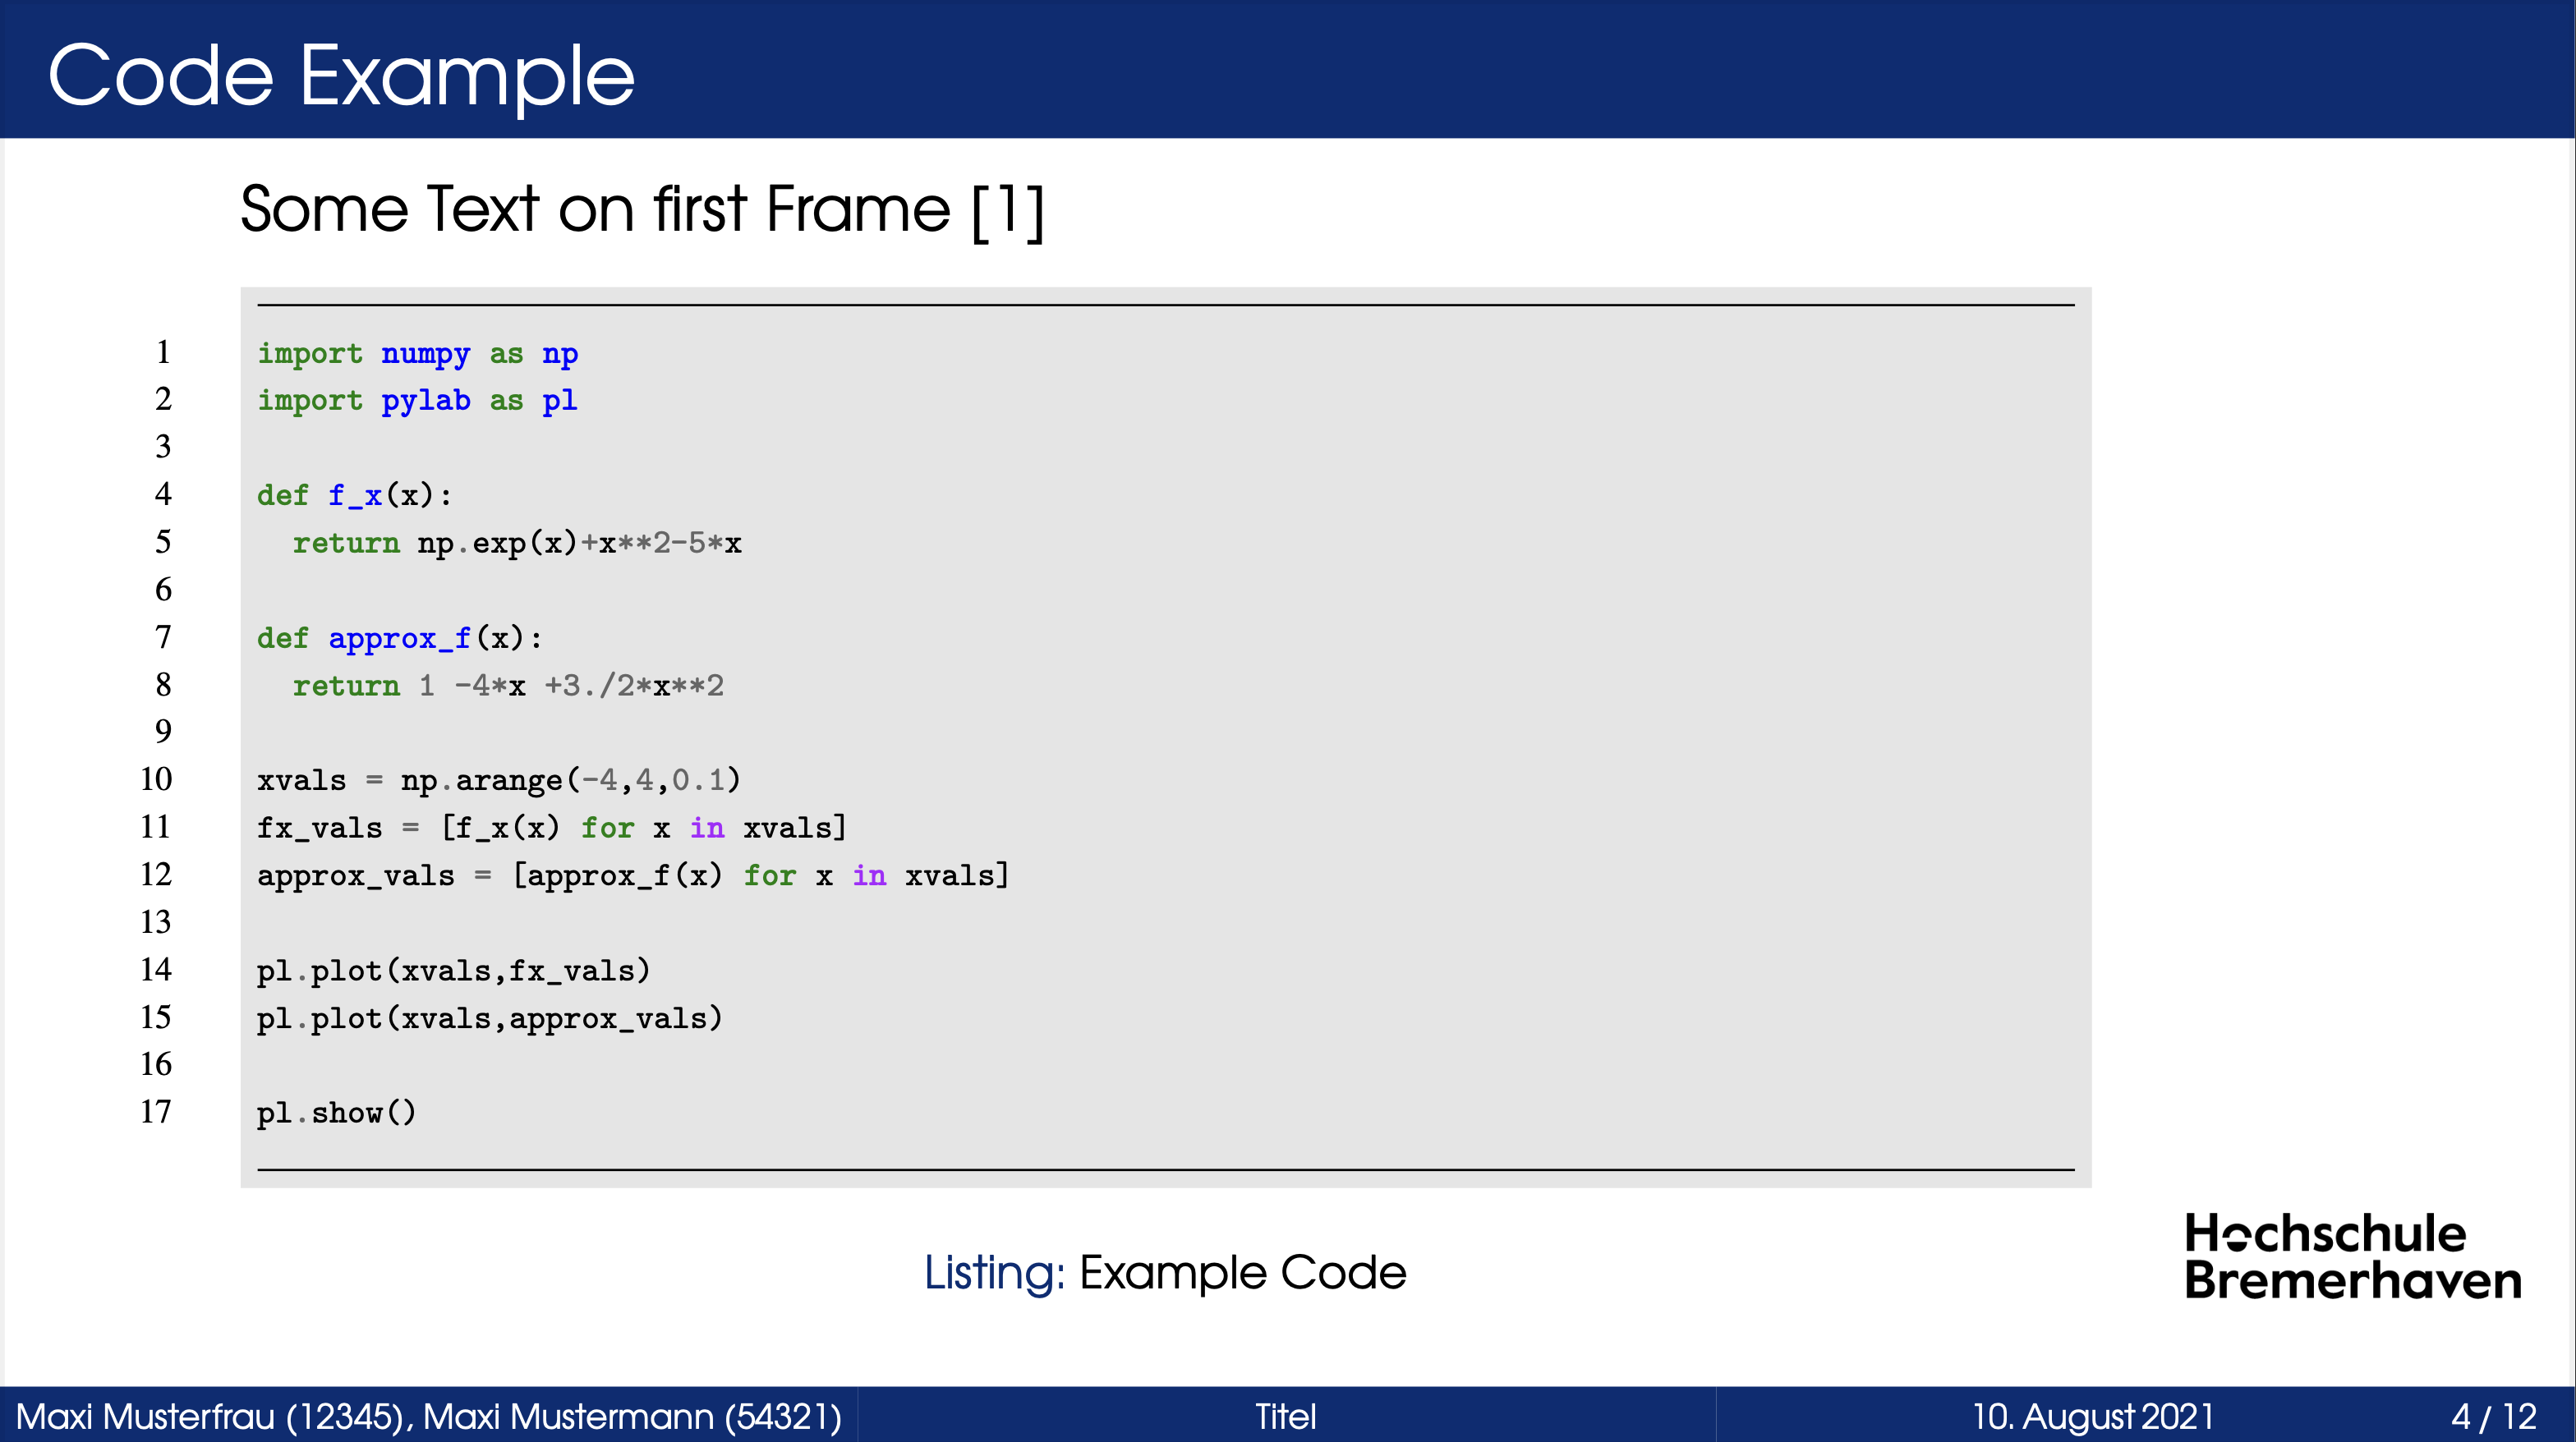
\includegraphics[width=0.9\textwidth]{src/abbildungen/beamer_frame.png}
	\caption{Frame mit Listing}
\end{figure}
\FloatBarrier


\newpage

\subsection{Quickbuild}

Wird ein Projekt mit der Zeit relativ groß, verfügt also über eine Vielzahl von
Listings, Tabellen, Abbildungen und Text, dann wird für das Kompilieren eine nicht
unerhebliche Zeit benötigt. Um das ganze Dokument, inkl. aller Referenzen und
Abkürzungen etc. zu bauen, ist dies auch nötig und lässt sich nicht vermeiden.
Oft benötigt man jedoch nur einen kurzen Blick auf Layout oder den Umfang des bisher
geschriebenen und möchte nicht das Dokument in seiner Gesamtheit kompilieren.\\
Für diese Anforderungen gibt es sog. \texttt{subfiles}, diese ermöglichen es, nur
einen kleinen Teil des Dokumentes zu kompilieren und als PDF zu betrachten. Dabei
kommt es zu gewissen Einschränkungen, so werden Seitenzahlen, Referenzen und Abkürzungen
nicht korrekt dargestellt, dennoch erhält man einen guten Blick auf das Layout.
Um mit \texttt{subfiles} zu arbeiten, muss einiges beachtet werden.
So muss statt des \texttt{\textbackslash input\{\}} das Kommando \texttt{\textbackslash subfile\{\}}
genutzt werden. Darüber hinaus müssen alle \texttt{.tex}-Dateien mit einer eigenen \texttt{documentclass}
ausgestattet werden. In der \texttt{hauptdatei.tex} sieht dies dann folgendermaßen aus.

\begin{code}{Einbinden von subfiles}{einbinden_subfiles}
\begin{minted}{latex}
	\subfile{src/einleitung.tex}
	\subfile{src/struktur.tex}
	\subfile{src/zurhauptdatei.tex}
\end{minted}
\end{code}

Jedes Subfile muss dann mit der passenden \texttt{documentclass} beginnen. 

\begin{code}{Erstellen von subfiles}{erstellen_subfiles}
\begin{minted}{latex}
	\documentclass[../hauptdatei.tex]{subfiles}
	\begin{document}
	\section{Beispiel}

	Hier könnte sinnvoller Inhalt stehen. 

	\end{document}
\end{minted}
\end{code}

Durch die eigene \texttt{documentclass}, welche wiederum auf die \texttt{hauptdatei.tex} verweist und 
die Angabe von \texttt{\textbackslash begin} bzw. \texttt{\textbackslash end\{document\}} kann die entsprechende 
\texttt{tex}-Datei separat kompiliert werden. Dafür kann das Skript \texttt{quickbild.sh} genutzt werden, welches 
als Argument den Namen der zu kompilierenden Datei erwartet und ein PDF erzeugt.\\
Abbildungen, Listings, Tabellen können wie gewohnt genutzt werden. Wird \texttt{buildlualatex.sh} ausgeführt, 
baut nach wie vor das gesamte Dokument inkl. aller Subfiles und Referenzen. 

\subsection{Prototyp-Dokumentation}

% Architektur-Diagramme (z. B. UML-Diagramme: Klassen-, Sequenz- oder Komponenten-Diagramme)
% Screenshots der Anwendung
% Falls vorhanden: Quellcode-Ausschnitte mit Erklärungen
\subsubsection{Überblick}

Dieser Prototyp wurde im Rahmen der Semesteraufgabe im Fach Qualitätsmanagement an der Hochschule Bremerhaven entwickelt. Ziel des Projekts ist die Umsetzung einer Hausverwaltung mit folgenden Kernfunktionen:

\begin{itemize}
    \item Verwaltung von Gebäuden, Zählern und Ablesewerten
    \item Verbrauchsanzeige mit historischen Daten (12 Monate)
    \item Speicherung und Validierung von Ablesedaten
    \item Visuelle Darstellung des Verbrauchs mit separaten Diagrammen für aktuelle und historische Werte
\end{itemize}

Das Projekt wurde als \textbf{Web-Anwendung mit Flask (Python)} umgesetzt. Als Datenspeicher werden \textbf{JSON-Dateien} genutzt, da der Fokus auf einem Prototyp und nicht auf einer produktiven Umgebung liegt.

\subsubsection{Architektur und Technologien}

Die Architektur folgt einem klassischen **MVC-Modell (Model-View-Controller)** mit folgenden Komponenten:

\begin{itemize}
    \item \textbf{Flask (Backend)} – Verarbeitung von Anfragen, Laden und Speichern der JSON-Daten
    \item \textbf{HTML + Jinja (Frontend)} – Dynamische Darstellung der Gebäude, Zähler und Verbrauchswerte
    \item \textbf{Matplotlib} – Visualisierung des Verbrauchs in Diagrammen
    \item \textbf{JavaScript} – Interaktive Formulare und automatische Aktualisierung der Gebäudeauswahl
\end{itemize}

\subsubsection{UML-Klassendiagramm}

\begin{figure}[h]
    \centering
    \includegraphics[width=0.7\textwidth]{uml_klassendiagramm.png}
    \caption{UML-Klassendiagramm der wichtigsten Entitäten}
\end{figure}

Das Klassendiagramm zeigt die Hauptklassen:
\begin{itemize}
    \item \texttt{Gebäude} – Beinhaltet Name, Adresse und Eingänge
    \item \texttt{Zähler} – Gehört zu einem Gebäude, speichert Typ und ID
    \item \texttt{Ablesung} – Speichert Werte mit Datum für einen bestimmten Zähler
\end{itemize}

\subsubsection{Sequenzdiagramm: Ablesung hinzufügen}

\begin{figure}[h]
    \centering
    \includegraphics[width=0.7\textwidth]{uml_sequenzdiagramm.png}
    \caption{UML-Sequenzdiagramm für das Hinzufügen einer Ablesung}
\end{figure}

\textbf{Ablauf:}
\begin{enumerate}
    \item Der Nutzer gibt eine Zähler-ID, ein Datum und einen Verbrauchswert ein.
    \item Das System überprüft die Zähler-ID und validiert die Eingabe.
    \item Die Ablesung wird gespeichert, wenn sie gültig ist.
    \item Die Verbrauchsanzeige wird aktualisiert.
\end{enumerate}

\subsubsection{Code-Struktur und wichtige Komponenten}

\textbf{Flask Backend (Python)}

\begin{code}{Flask Backend (Python)}{Verbrauchsanzeige}
    \begin{minted}{python}
        @app.route("/zaehler/hinzufuegen", methods=["POST"])
        def zaehler_hinzufuegen():
            zaehler = load_json(ZAEHLER_FILE)
            neue_id = f"{request.form['gebaeude_id']}-{datetime.now().year}-{random.randint(1000,9999)}"
            neuer_zaehler = {"id": neue_id, "gebaeude_id": request.form["gebaeude_id"], "typ": request.form["typ"]}
            zaehler.append(neuer_zaehler)
            save_json(ZAEHLER_FILE, zaehler)
            return redirect("/zaehler")
    \end{minted}
\end{code}



\begin{code}{HTML-Frontend mit Jinja}{Frontend}
    \begin{minted}{html}
        <form method="POST" action="/ablesung/hinzufuegen">
            <label>Zähler-ID:</label>
            <input type="text" name="zaehler_id" required>
            <label>Datum:</label>
            <input type="date" name="datum" required>
            <label>Wert:</label>
            <input type="number" name="wert" required>
            <button type="submit">Ablesung speichern</button>
        </form>
    \end{minted}
\end{code}

\begin{code}{Matplotlib Diagramm-Erstellung}{Bildgenerierung}
    \begin{minted}{python}
        plt.figure(figsize=(10, 5))
        for zaehler_id in set(a["zaehler_id"] for a in ablesungen):
            daten = sorted([a for a in ablesungen if a["zaehler_id"] == zaehler_id], key=lambda x: x["datum"])
            x = [datetime.strptime(a["datum"], "%Y-%m-%d") for a in daten]
            y = [a["wert"] for a in daten]
            plt.plot(x, y, marker="o", linestyle="-", label=f"Zähler {zaehler_id}")
        plt.legend()
        plt.savefig("static/verbrauchsdiagramm.png")
    \end{minted}
\end{code}

\subsubsection{Zusammenfassung und Fazit}

Der Prototyp bietet eine funktionale Umsetzung der Anforderungen mit einer benutzerfreundlichen Verwaltung von Gebäuden, Zählern und Verbrauchswerten. Die Nutzung von Flask und JSON für die Datenhaltung macht ihn leicht erweiterbar.

\textbf{Hauptmerkmale:}
\begin{itemize}
    \item Dynamische Verwaltung von Gebäuden und Zählern
    \item Historische Verbrauchsanzeige mit separaten Diagrammen
    \item Farblich unterscheidbare Zähler-Darstellung
    \item Integration der letzten 12 Monate in die Diagramme
\end{itemize}

Mögliche Erweiterungen wären eine Umstellung auf eine Datenbank sowie eine Nutzerverwaltung für Admin- und Standardbenutzerrechte.
\newpage

% Selbstständigkeits Erklärung
\phantomsection
\addcontentsline{toc}{section}{Selbstständigkeitserklärung}

% Header für Erklärung
\ohead{Selbstständigkeitserklärung}

% Input Erklärung
\section*{Selbstständigkeitserklärung}

%\vspace{1cm}
Wir versichern, die von uns vorgelegte Arbeit selbstständig verfasst zu haben. Alle Stellen, die wörtlich oder sinngemäß aus veröffentlichten oder nicht veröffentlichten Arbeiten anderer entnommen sind, 
haben wir als entnommen kenntlich gemacht. Sämtliche Quellen und Hilfsmittel, die wir für die Arbeit benutzt haben, sind angegeben. Die Arbeit haben wir mit gleichem Inhalt bzw. in wesentlichen 
Teilen noch keiner anderen Prüfungsbehörde vorgelegt.

\vspace*{1cm}

\begin{tblr}{X[l] X[l]}
Bremerhaven, den \today & Unterschrift:\\
\end{tblr}

% Leere Abschlussseite
%\newpage
%\thispagestyle{empty} % erzeugt Seite ohne Kopf- / Fusszeile
%\mbox{}

\end{document}
